\chapter{Precipitação total}\label{cap:resultados_tp}
A precipitação associada a ciclones extratropicais complementa o vento (Capítulo~\ref{cap:resultados_wind10}) na caracterização estrutural do sistema. Diferentemente do vento, ela integra processos de calor, desde a condensação estratiforme de grande escala até a convecção embutida de mesoescala ligada à liberação de calor latente (Seção~\ref{subsec:tb_modelos}).
Este capítulo estabelece a estrutura espacial da precipitação durante as fases do ciclo de vida dos ciclones extratropicais do Atlântico Sul-Ocidental, seguindo a progressão metodológica do Capítulo~\ref{cap:resultados_wind10}: (i)~evolução das distribuições de magnitude segundo a intensidade do vórtice e a região de gênese; (ii)~localização espacial preferencial dos máximos de precipitação; e (iii)~decomposição EOF.
A Seção~\ref{sec:pdf_tp} examina as PDF de magnitude; as Seções~\ref{subsec:kde_tp_global} e~\ref{subsec:kde_tp_p90}, a distribuição espacial dos máximos (PDFe); e as Seções~\ref{subsec:var_exp_tp}--\ref{sec:dinamica_pc1_tp}, a estrutura modal via EOF.
Os resultados são contrastados com os do campo de vento para avaliar, no Capítulo~\ref{chap:meof}, se ambas as variáveis compartilham uma organização espacial coerente.

% --- SEÇÃO PRINCIPAL: PDF DE PRECIPITAÇÃO TOTAL ---

\section{Distribuição de magnitudes (PDF)}\label{sec:pdf_tp}

\begin{figure}[htbp]
\centering
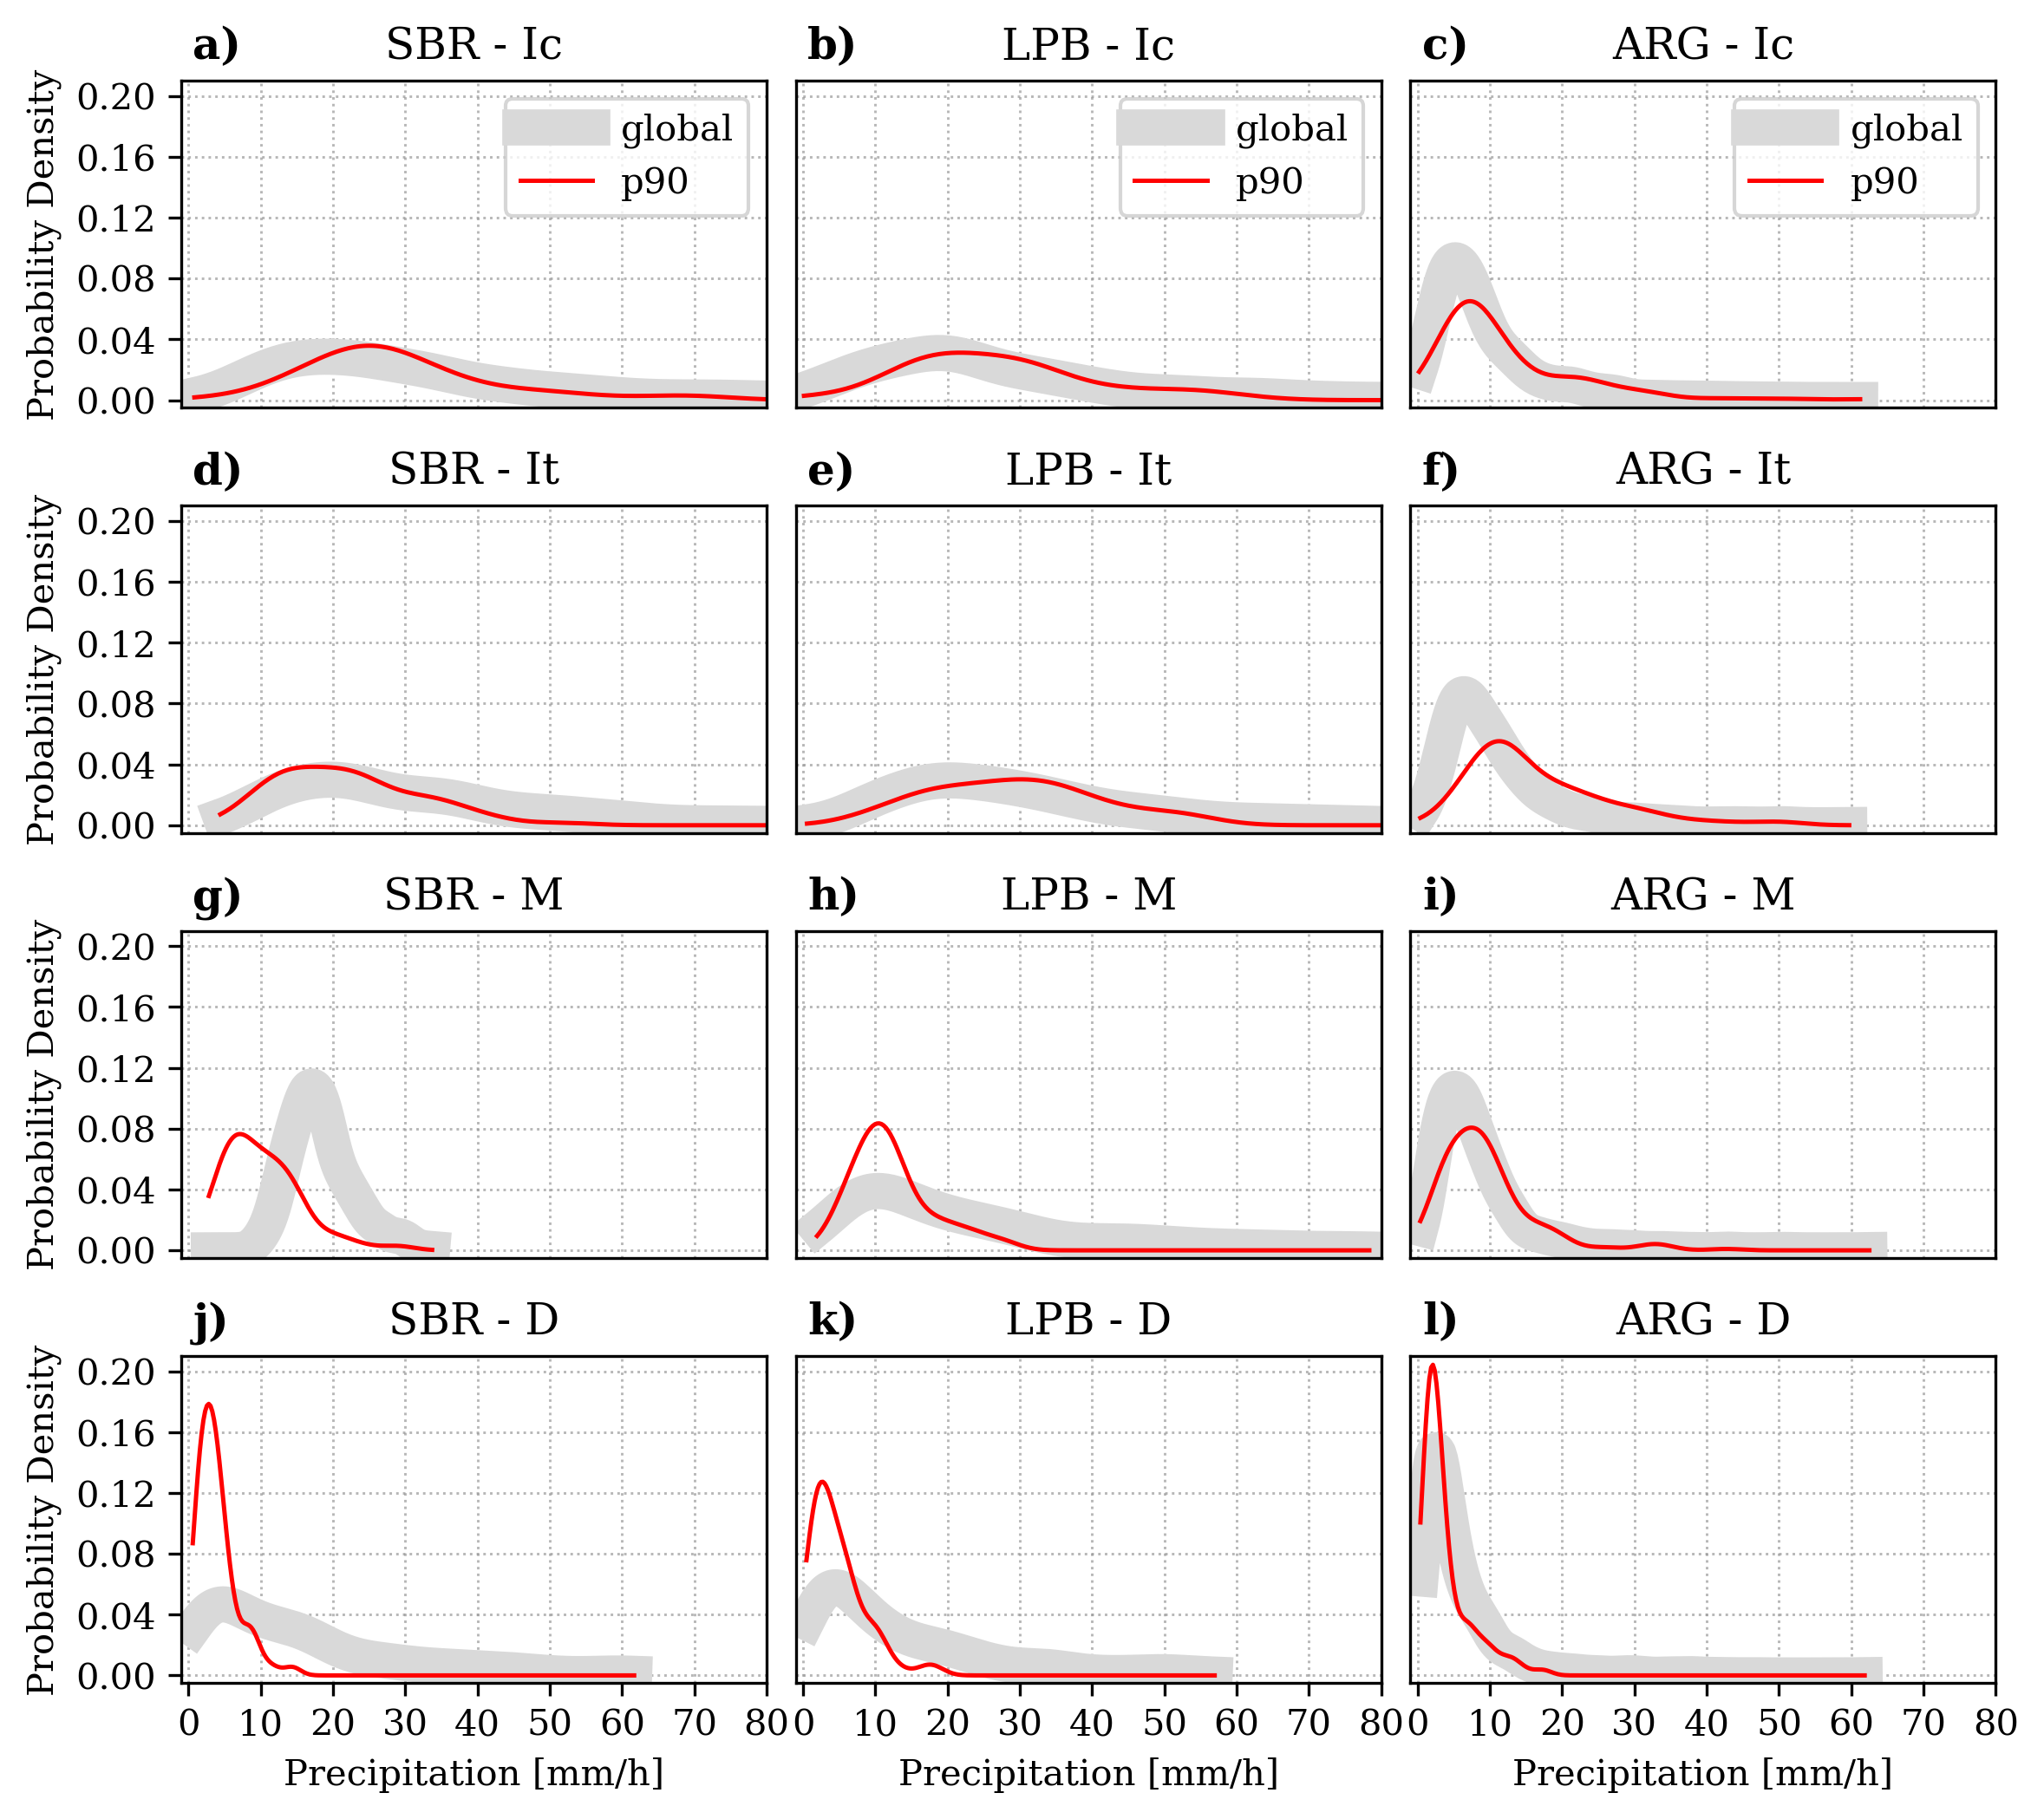
\includegraphics[width=\textwidth]{images/tp/PDF_tp_sigma025.png}
\caption[PDF de magnitudes máximas de precipitação total]{Funções de densidade de probabilidade (PDF) para as magnitudes máximas de precipitação total (mm/h). As colunas indicam a região de ciclogênese (SBR, LPB, ARG) e as linhas a evolução através das fases do ciclo de vida (Ic, It, M, D). Contrasta-se a População Global (referência, sombreado cinza) com o subconjunto dos máximos de vorticidade relativa em 850 hPa alcançados em seu ciclo de vida: p90 (ciclones intensos, linha vermelha).}
\label{fig:pdf_tp}
\end{figure}

A Figura~\ref{fig:pdf_tp} mostra a distribuição estatística dos máximos espaciais de precipitação (mm/h) para os compostos do instante central de cada fase, estratificados por região de ciclogênese (SBR, LPB, ARG) e pelo pico de vorticidade relativa em 850 hPa alcançado no ciclo de vida (p90).
Os ciclones extratropicais são a principal causa de precipitação em latitudes médias, e em simulações idealizadas os ciclones com maior vorticidade máxima produzem mais precipitação, embora essa relação seja fraca nos ciclones de latitudes altas com pouca umidade \citep{sinclair2023relationship}. A comparação entre a População Global e p90 permite avaliar se essa relação se cumpre nas regiões de estudo.
Esses campos foram extraídos dentro do domínio centrado no núcleo de cada sistema, seguindo a metodologia aplicada ao vento (Capítulo~\ref{cap:resultados_wind10}).

Nas fases incipiente e intensificação (painéis a, b, d e e), SBR e LPB mostram na População Global um perfil plano e estendido com pico modal próximo de 20~mm/h, reflexo da ampla dispersão de intensidades nessas regiões.
Em SBR e LPB, a distribuição de p90 é parecida com a da População Global da qual faz parte, embora seu pico se desloque para valores um pouco maiores em SBR durante a fase incipiente (${\sim}$25~mm/h) e em LPB durante a intensificação (${\sim}$30~mm/h). As taxas superiores a 60~mm/h aparecem com densidades muito baixas e não são mais frequentes em p90 do que na População Global, portanto não são exclusivas dos ciclones mais intensos.
No ERA5, a precipitação total é a soma da componente de grande escala e da convectiva parametrizada, e nos ciclones mais intensos é subestimada em torno de 23\% \citep{chen2024evaluation}, o que deve ser levado em conta ao interpretar os valores absolutos (Seção~\ref{sec:datos_era5}). Em ciclones do Mediterrâneo, \citet{flaounas2018heavy} encontram que as taxas mais altas (mais de 50~mm em 3~h) se devem com maior probabilidade à convecção profunda do que à Cinta Transportadora Quente (WCB, \textit{warm conveyor belt}), embora uma parte importante dessa convecção esteja embutida no WCB. Nesses ciclones, a chuva convectiva ocorre perto do centro e em seu lado leste, e a do WCB em direção ao nordeste, o que no Hemisfério Sul corresponderia ao sudeste.

Em ARG (painéis c e f), a População Global apresenta um pico pronunciado em valores baixos (${\sim}$5--6~mm/h, densidade ${\sim}$0.10) e uma queda rápida em direção a valores maiores, compatível com a menor disponibilidade de umidade em latitudes mais altas \citep{sinclair2023relationship}.
Em p90, o pico da fase incipiente se mantém em valores semelhantes, com menor densidade, enquanto na intensificação (painel f) se desloca para ${\sim}$11~mm/h, com mais casos entre 15 e 35~mm/h do que na População Global. É a separação mais clara entre p90 e a População Global nas fases iniciais, embora seus valores permaneçam muito abaixo dos de SBR e LPB.

Ao alcançar a maturidade (painéis g--i) e o decaimento (painéis j--l), as diferenças entre a População Global e p90 aumentam.
Na maturidade, a População Global de SBR apresenta um pico estreito próximo de 17~mm/h, enquanto p90 se desloca para ${\sim}$7~mm/h. Em LPB ambas têm seu pico próximo de 10~mm/h, mas a curva de p90 é mais aguda. No decaimento, a População Global de ambas as regiões se desloca para ${\sim}$5~mm/h e p90 se concentra em valores mínimos (1--4~mm/h), com densidades de ${\sim}$0.18 em SBR e ${\sim}$0.13 em LPB.
Em ARG, o decaimento (painel l) apresenta a distribuição mais concentrada da figura. O pico de p90 se localiza próximo de 2~mm/h, com uma densidade de ${\sim}$0.20, superior à de SBR e LPB, e a densidade de ambas as curvas tende a zero acima de ${\sim}$20~mm/h. Nessa fase, os ciclones de ARG produzem quase exclusivamente precipitação de baixa intensidade.

Em contraste, ARG apresenta precipitações menores em todas as fases. Isso concorda com \citet{gramcianinov2019properties}, que, a partir da precipitação média em um raio de 6° ao redor do centro, encontram que os ciclones de SBR e LPB produzem a precipitação mais intensa, com distribuições semelhantes entre ambas as regiões, enquanto em ARG são menos os ciclones que superam os 20~mm/dia. Essa diferença é coerente com o maior peso dos processos úmidos em SBR e LPB e da baroclinicidade de grande escala em ARG (Seções~\ref{subsec:tb_sbr}, \ref{subsec:tb_lpb} e~\ref{subsec:tb_arg}).

Em p90, a precipitação diminui na maturidade, fase que contém o instante de máxima intensidade para a maioria dos ciclones (Tabela~\ref{tab:fase_max_intensidad}). Essa defasagem coincide com \citet{dacre2023climatology}, que, para os 400 ciclones mais intensos segundo a vorticidade a 850~hPa nos oceanos ao redor da Austrália (maio a setembro, 1979--2021), encontram que o máximo de precipitação ocorre em média 24~h antes da intensidade máxima. Os autores explicam isso pela menor disponibilidade de umidade à medida que o ciclone se desloca em direção ao polo, ou pelo aquecimento diabático da fase de máxima precipitação, que reforça a intensidade do ciclone. Em ${\sim}$5000 ciclones invernais do Atlântico Norte, \citet{heitmann2024lifecycle} encontram que a taxa e o volume de precipitação do WCB alcançam seu máximo enquanto o ciclone ainda está se aprofundando, antes de alcançar sua pressão mínima.
Também coincide com \citet{mcerlich2023extremes}, que, em compostos de ciclones de latitudes médias do Hemisfério Sul com ERA5, encontram que a precipitação extrema ocorre com mais frequência durante o aprofundamento, antes do pico de intensidade, e que na fase de decaimento sua frequência e sua contribuição à precipitação total caem para 46\% e 80\% do valor do aprofundamento, respectivamente. Os mesmos autores encontram que a precipitação extrema se concentra em uma região menor ao redor do centro do que a precipitação não extrema.

Essa diminuição também poderia estar relacionada à chegada de ar subsidente e seco perto do centro. Em um ciclone do Hemisfério Norte com seclusão quente, \citet{shapiro1999bridge} documentam subsidência a oeste do centro e precipitação deslocada para leste, adiante da frente fria. A localização dos máximos de precipitação em relação ao centro é analisada na Seção~\ref{sec:pdfe_tp}.

% --- SEÇÃO PRINCIPAL: PDFe ESPACIAL DE PRECIPITAÇÃO ---

\section{Distribuição espacial de máximos (PDFe)}\label{sec:pdfe_tp}

\subsection{População Global}\label{subsec:kde_tp_global}

\begin{figure}[htbp]
\centering
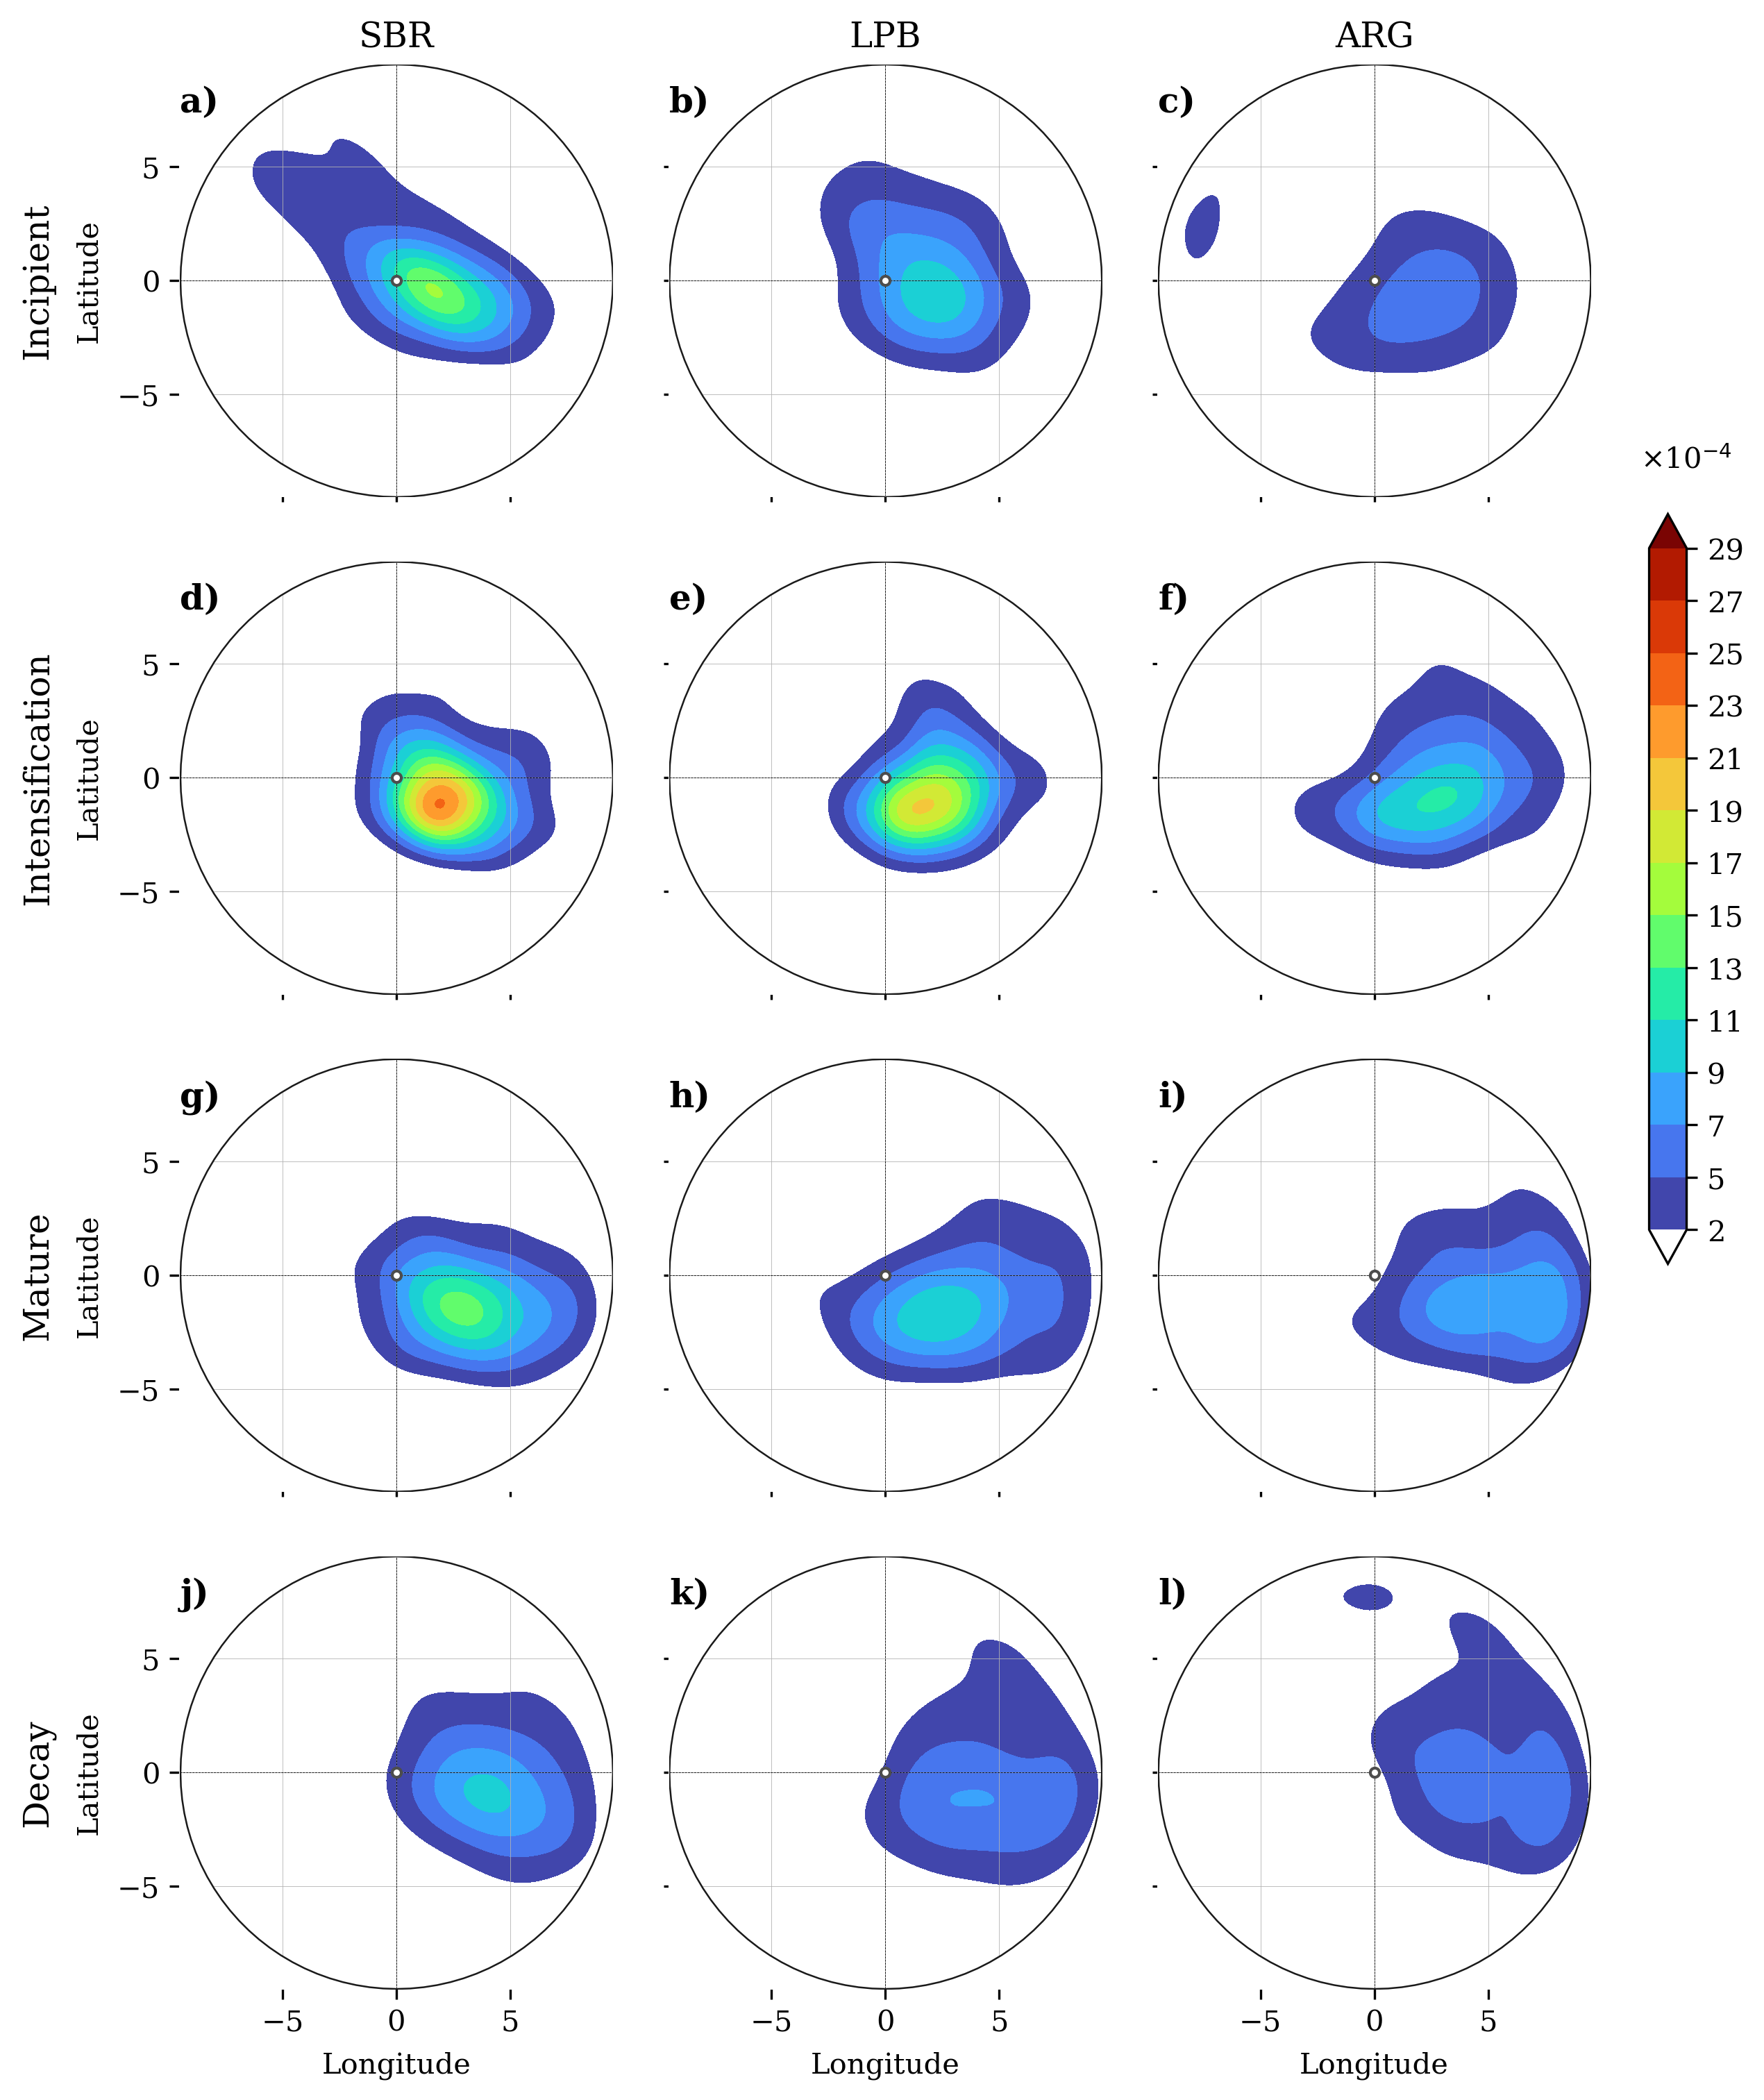
\includegraphics[width=\textwidth]{images/tp/kde_tp_global_fasesxreg.png}
\caption[PDF espacial de precipitação máxima (População Global)]{Estimação de densidade espacial bidimensional (usando estimação de densidade por kernel KDE) para a localização geométrica dos máximos de precipitação total (mm/h) na População Global de referência. A matriz organiza a evolução espacial através das fases evolutivas Incipiente (a-c), Intensificação (d-f), Maturidade (g-i) e Decaimento (j-l), segregadas pelas regiões de ciclogênese SBR, LPB e ARG. O domínio abrange $20^{\circ} \times 20^{\circ}$ com centro no vórtice $(0,0)$. A barra de cores quantifica a densidade de probabilidade relativa escalada por $10^{-4}$.}
\label{fig:kde_tp_global}
\end{figure}

A Figura~\ref{fig:kde_tp_global} mostra a densidade espacial da localização dos máximos de precipitação para a População Global.
Como no vento (Seção~\ref{sec:kde_espacial_global}), na fase incipiente os máximos se localizam a leste do centro, embora a precipitação apresente uma assimetria mais pronunciada.

Em SBR (painel a), a densidade máxima (${\approx}$\,15--17\,$\times10^{-4}$) se localiza a ${\sim}$2° a leste do centro, quase na sua mesma latitude, com uma cauda em direção ao noroeste, que é a assimetria mais notável dessa fase. LPB (painel b) apresenta um núcleo em posição similar e de menor densidade (${\approx}$\,9--11\,$\times10^{-4}$), com elongação ao norte. Em ARG (painel c), o núcleo principal se localiza a leste-sudeste (${\approx}$\,5--7\,$\times10^{-4}$) e coexiste com um foco secundário pequeno e fraco no noroeste.

A intensificação concentra as maiores densidades. Em SBR (painel d), o núcleo alcança ${\approx}$\,23--25\,$\times10^{-4}$, o máximo da figura, e se localiza a ${\sim}$2° a leste e ${\sim}$1° ao sul do centro, com contornos internos quase circulares. LPB (painel e) apresenta um núcleo na mesma posição (${\approx}$\,19--21\,$\times10^{-4}$), com a envoltória estendida em direção ao nordeste. ARG (painel f) tem a menor densidade dessa fase (${\approx}$\,11--13\,$\times10^{-4}$), com o núcleo a leste-sudeste, uma extensão em direção ao nordeste e sem o foco secundário da fase incipiente.

ARG apresenta a menor densidade da linha nas quatro fases (painéis c, f, i e l), o que é coerente com a menor precipitação dessa região descrita na Seção~\ref{sec:pdf_tp}.

Ao alcançar a maturidade, as densidades diminuem e os padrões se alargam. Em SBR (painel g), o núcleo (${\approx}$\,13--15\,$\times10^{-4}$) se localiza a ${\sim}$3° a leste e ${\sim}$1.5° ao sul do centro, com forma ovalada de eixo oeste-noroeste a leste-sudeste. LPB (painel h) apresenta um núcleo em posição semelhante (${\approx}$\,9--11\,$\times10^{-4}$), com contornos que se estendem em direção ao leste e ao nordeste. ARG (painel i) tem a menor densidade (${\approx}$\,7--9\,$\times10^{-4}$) e o núcleo mais afastado em direção ao leste da linha (${\sim}$6°). Diferentemente do vento, cujos máximos se deslocam nessa fase para o quadrante noroeste (Seção~\ref{sec:kde_espacial_global}), os máximos de precipitação permanecem a leste e sudeste do centro.

No decaimento, as densidades são baixas e os máximos se localizam mais distantes do centro, a ${\sim}$4--6° a leste, sem densidade apreciável a oeste do centro em nenhuma região. SBR (painel j) registra sua menor densidade (${\approx}$\,9--11\,$\times10^{-4}$), com os contornos restritos à metade oriental do domínio. LPB (painel k) apresenta um núcleo pequeno a leste-sudeste (${\approx}$\,7--9\,$\times10^{-4}$), com contornos que se estendem em direção ao nordeste. Em ARG (painel l), o núcleo se localiza a leste (${\approx}$\,5--7\,$\times10^{-4}$, junto com a fase incipiente a menor densidade da figura), com um foco isolado e fraco no extremo norte do domínio.

A localização dos máximos a leste e sudeste do centro na População Global coincide com a que a literatura atribui à precipitação do WCB. No modelo conceitual de \citet{browning1986conceptual}, o WCB ascende adiante da frente fria e sobre a frente quente, no setor quente do ciclone. Em compostos de precipitação média de ciclones oceânicos de ambos os hemisférios, \citet{naud2020evaluation} situam o máximo a ${\sim}$250~km do centro, em direção ao polo e a leste, e um mínimo a oeste, o que no Hemisfério Sul corresponde ao sudeste. Em SBR e LPB, os núcleos das fases incipiente e intensificação se localizam a uma distância semelhante (${\sim}$2° a leste e 0.5--1.3° ao sul), e a oeste do centro a densidade é baixa, exceto a cauda noroeste da fase incipiente.
Em escala global, \citet{catto2015fronts} encontram que, em partes das latitudes médias, mais de 60\% dos eventos de precipitação extrema coincidem com frentes, até 90\% deles associados a um WCB, e que as frentes com WCB têm entre 2 e 10 vezes mais probabilidade de produzir precipitação extrema do que as frentes sem WCB.

As maiores densidades de SBR e LPB poderiam estar relacionadas ao transporte de umidade desde latitudes tropicais ao longo do flanco oriental do ciclone em níveis baixos, que \citet{vera2002cold} documentam para as ondas sinóticas da estação fria sobre a América do Sul subtropical e que favorece a precipitação no sudeste do continente.

Na maturidade e no decaimento (painéis g--l), os máximos permanecem a leste do centro, mas se afastam dele e se dispersam. Como a População Global inclui os ciclones p90, a seção seguinte examina se os ciclones mais intensos se afastam desse padrão.

\subsection{Subconjunto de ciclones intensos p90}\label{subsec:kde_tp_p90}

\begin{figure}[htbp]
\centering
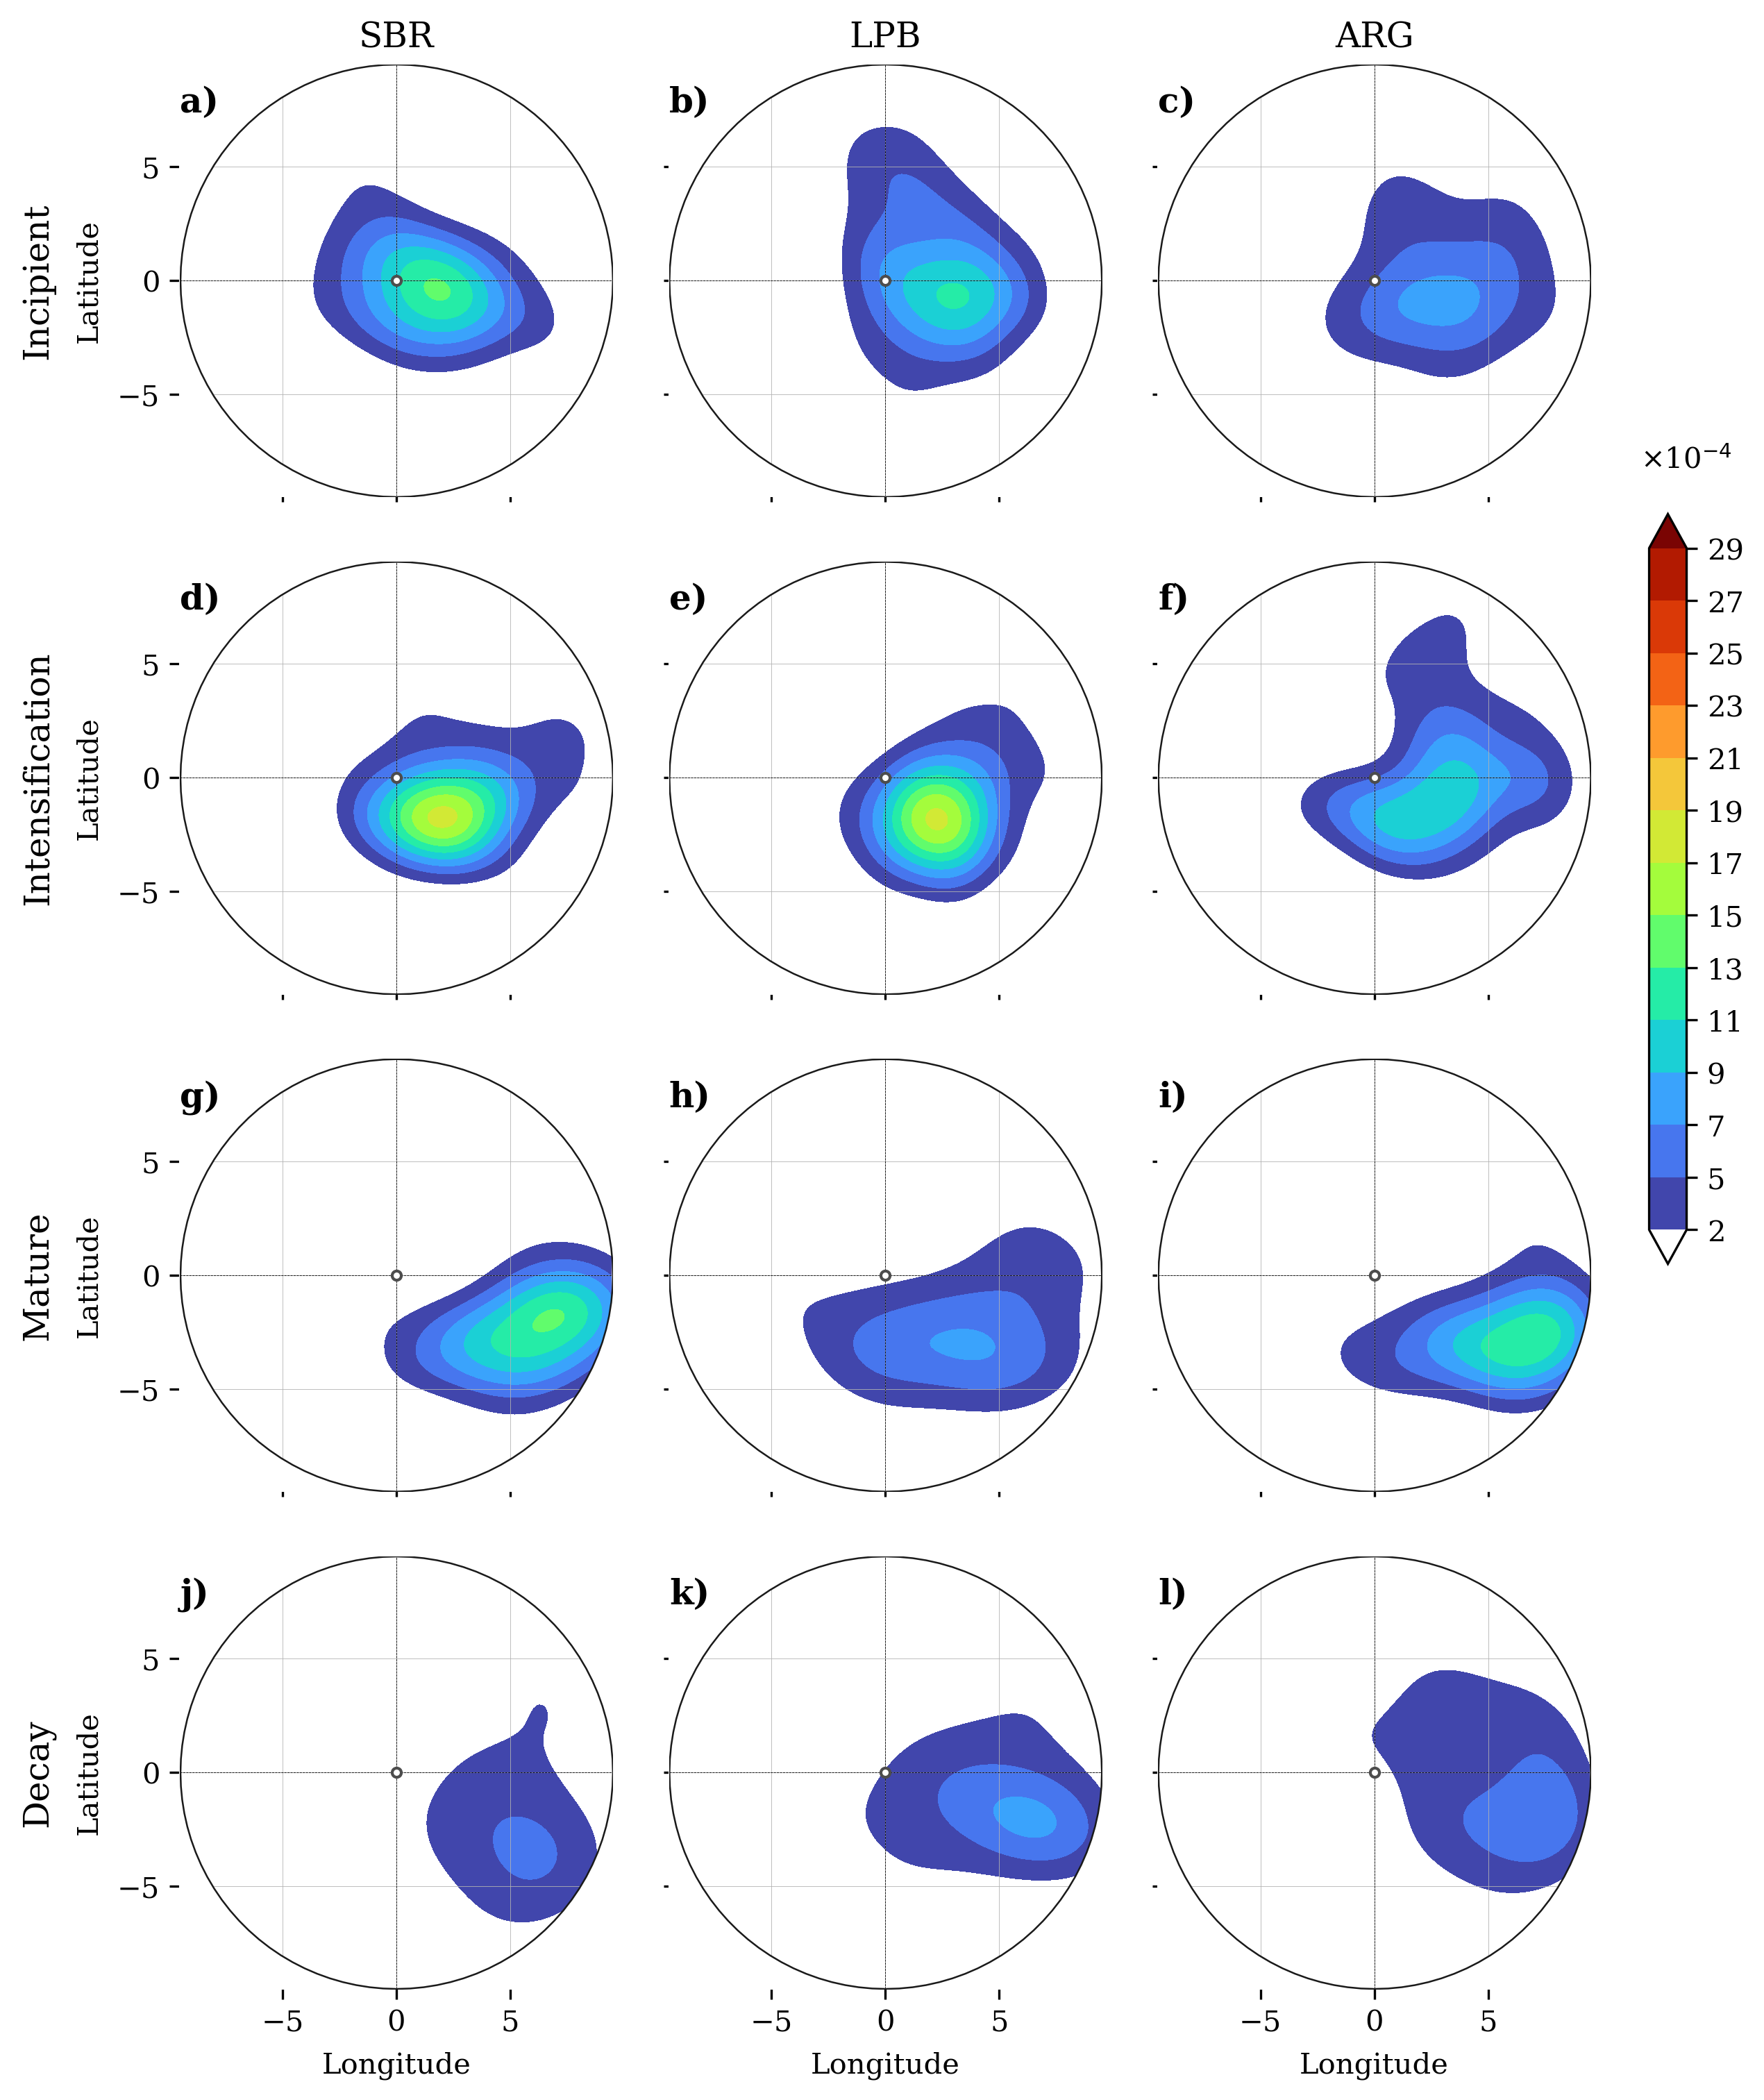
\includegraphics[width=\textwidth]{images/tp/kde_tp_p90_fasesxreg.png}
\caption[PDF espacial de precipitação máxima (subconjunto p90)]{Estimação de densidade espacial bidimensional (PDFe) para a localização geométrica dos máximos de precipitação total (mm/h) correspondente ao subconjunto de ciclones intensos (percentil 90). O formato dos painéis (a--l), a evolução temporal, a segregação regional e a escala colorimétrica ($10^{-4}$) replicam a estrutura da Figura~\ref{fig:kde_tp_global}, para facilitar a comparação com a População Global.}
\label{fig:kde_tp_p90}
\end{figure}

A Figura~\ref{fig:kde_tp_p90} mostra a mesma densidade para o subconjunto p90. Nas fases incipiente e intensificação, os máximos de p90 se localizam em posições semelhantes às da População Global, a ${\sim}$2--3° a leste e sudeste do centro. A partir da maturidade, por sua vez, os núcleos de p90 se afastam mais do centro e se deslocam mais para o sul do que os da População Global, até ${\sim}$6--7° a leste em SBR e ARG, e adotam formas alongadas na direção oeste-sudoeste a leste-nordeste.

Em SBR (painel a), a densidade máxima (${\approx}$\,13--15\,$\times10^{-4}$) se localiza a ${\sim}$2° a leste do centro, quase na sua mesma latitude, em um núcleo mais compacto do que o da População Global e sem a cauda noroeste. Em LPB (painel b), o núcleo (${\approx}$\,11--13\,$\times10^{-4}$) se localiza a ${\sim}$3° a leste-sudeste, com uma envoltória fraca que se estende em direção ao norte. Em ARG (painel c), o núcleo se localiza em uma posição semelhante (${\approx}$\,7--9\,$\times10^{-4}$) e não aparece o foco secundário do noroeste presente na População Global.

Como na População Global, a intensificação apresenta as maiores densidades de p90. Em SBR (painel d) e LPB (painel e), o núcleo alcança ${\approx}$\,17--19\,$\times10^{-4}$ e se localiza a ${\sim}$2° a leste e ${\sim}$2° ao sul do centro, na mesma posição que na População Global, embora com menor densidade em SBR (${\approx}$\,23--25\,$\times10^{-4}$ na População Global). ARG (painel f) apresenta a menor densidade da linha (${\approx}$\,9--11\,$\times10^{-4}$), com o núcleo a leste-sudeste e uma envoltória que se estende em direção ao norte e ao nordeste.

Na maturidade, os núcleos de p90 se afastam do centro e adotam formas alongadas na direção oeste-sudoeste a leste-nordeste, sem máximos no centro nem no noroeste. Em SBR (painel g), o núcleo (${\approx}$\,13--15\,$\times10^{-4}$) se localiza a ${\sim}$6--7° a leste e ${\sim}$2° ao sul do centro, perto da borda do domínio e mais distante do centro do que na População Global. LPB (painel h) apresenta a menor densidade da linha (${\approx}$\,7--9\,$\times10^{-4}$) e o núcleo mais ao sul (${\sim}$3.5° a leste e ${\sim}$3° ao sul), dentro de uma faixa larga que se estende até $+$9° de longitude. ARG (painel i) apresenta uma faixa semelhante à de SBR (${\approx}$\,11--13\,$\times10^{-4}$), com o núcleo a ${\sim}$6.5° a leste e ${\sim}$3° ao sul. Essa extensão é semelhante à que \citet{flaounas2018heavy} encontram em ciclones do Mediterrâneo 12~h após a máxima intensidade, quando a chuva associada ao WCB forma uma faixa que se estende de 2.5° a oeste até 10° a leste do centro, com mais de 40\% dos casos em direção ao polo, o que no Hemisfério Sul corresponde ao sul do centro.

% [Comentado na revisão 2026-09-30: Naud 2025 não dá localização em relação ao centro e a tese não identifica oclusão; possível contraste futuro]
% Segundo \citet{naud2025lifecycle} para o Hemisfério Norte, os ciclones ocluídos desenvolvem uma crista térmica que conecta o centro do sistema com o vértice do setor quente, onde se maximiza a precipitação mediante um forçante de ascensão próprio na periferia. Ao alcançar sua máxima intensidade, os p90 intensificam a intrusão seca descrita na Seção~\ref{sec:pdf_tp} \citep{shapiro1999bridge}, que erradica a nebulosidade profunda do núcleo e abre o \textit{dry slot} característico.

No modelo de Shapiro-Keyser (Seção~\ref{subsec:tb_modelos}), os ciclones ocluídos apresentam ainda uma banda de precipitação enrolada (\textit{wrap-around precipitation}) no quadrante ocluso, produzida pela corrente do trowal, que se origina no setor quente \citep{martin1999forcing}. No Hemisfério Norte, essa precipitação se localiza ao norte e a oeste do mínimo de pressão, o que no Hemisfério Sul corresponderia ao sul e a oeste do centro. Em três ciclones invernais maduros da costa sul do Japão, \citet{sawada2021heavy} observam precipitação estratiforme extensa a leste do centro associada ao WCB, bandas convectivas perto do centro onde a intrusão seca se superpõe ao WCB, e precipitação estratiforme atrás do centro associada ao CCB. Os núcleos de p90 na maturidade, a leste e sudeste do centro, coincidem com a posição da precipitação associada ao WCB mais do que com a do quadrante ocluso.

No decaimento, os núcleos de p90 se localizam a leste-sudeste, a mais de 5° do centro, com densidades baixas. Em SBR (painel j), o núcleo (${\approx}$\,5--7\,$\times10^{-4}$) é menos denso do que na População Global (${\approx}$\,9--11\,$\times10^{-4}$) e se localiza mais ao sul. LPB (painel k) apresenta a maior densidade da linha (${\approx}$\,7--9\,$\times10^{-4}$), com o núcleo a ${\sim}$6° a leste e contornos que alcançam $+$9° de longitude. Em ARG (painel l), o núcleo (${\approx}$\,5--7\,$\times10^{-4}$) se localiza a ${\sim}$6.5° a leste, com uma envoltória que cobre quase todo o semicírculo oriental.

Na maturidade, os máximos de precipitação de p90, a ${\sim}$3.5--7° a leste e 2--3° ao sul do centro, se localizam no quadrante oposto ao dos máximos de vento de p90, que se concentram no noroeste, entre $-$1° e $-$3° de longitude e entre $+$1.5° e $+$3° de latitude (Seção~\ref{sec:kde_espacial_p90}). Essa separação já aparece na População Global (Seção~\ref{subsec:kde_tp_global}), mas é mais acentuada em p90, cujos máximos de precipitação se localizam mais longe do centro. A Seção~\ref{subsec:eof1_tp_p90} examina se essa separação se reflete também nos padrões de variabilidade.
% --- SEÇÃO: PADRÕES DOMINANTES DE VARIABILIDADE (EOF) - PRECIPITAÇÃO ---
\section{Organização estrutural: Análise EOF}\label{sec:eof_tp}

\subsection{Fracionamento de variância}\label{subsec:var_exp_tp}

\begin{figure}[htbp]
\centering
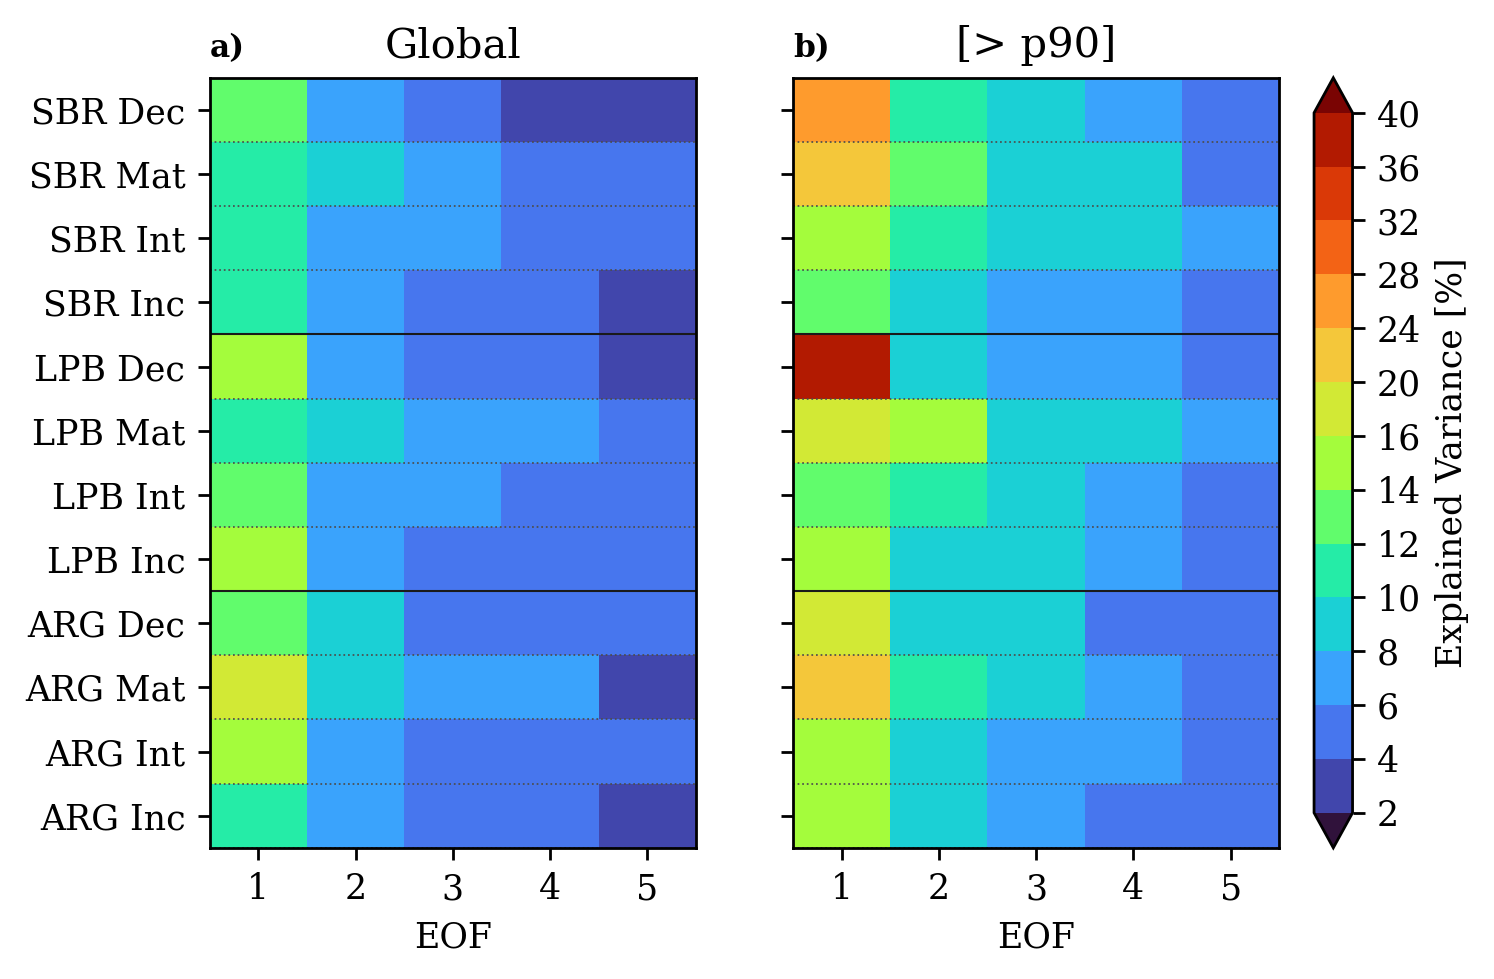
\includegraphics[width=0.8\textwidth]{images/tp/all_expvar_tp_mean2times.png}
\caption[Variância explicada pelos primeiros cinco modos (EOF1--EOF5) de precipitação]{Fracionamento da variância espacial total contida nos primeiros cinco modos dominantes (EOF1 a EOF5) do campo de precipitação total. Contrasta-se a distribuição da variância da População Global frente ao subconjunto de intensidade (p90) ao longo do ciclo de vida para cada região de ciclogênese.}
\label{fig:var_exp_tp}
\end{figure}

A Figura~\ref{fig:var_exp_tp} apresenta a distribuição percentual da variância espacial explicada pelos cinco primeiros modos empíricos (EOF1 a EOF5). As colunas contrastam a População Global (painel a) e o subconjunto de intensidade extrema (p90, painel b); as linhas correspondem às doze combinações de região de ciclogênese e fase evolutiva. A escala cromática quantifica a porcentagem de variância explicada. Os tons frios indicam modos dispersos; os quentes, alta concentração no modo principal.

Na População Global (painel a), o espectro de variância apresenta tons frios entre os cinco modos em todas as regiões e fases. O EOF1 explica entre 11.1\% e 16.4\% da variância total. Em SBR oscila entre 11.3\% (maturidade) e 13.8\% (decaimento), sem fase dominante. LPB apresenta seu máximo em incipiente (14.4\%) e decaimento (14.3\%), com a maturidade como mínimo (11.8\%). ARG exibe o comportamento mais distintivo. O EOF1 alcança seu máximo na maturidade (16.4\%), superando a intensificação (15.6\%), indicando um modo dominante bem diferenciado em relação a SBR e LPB. Os três primeiros modos explicam em conjunto, na maturidade, aproximadamente 26.8\% (SBR), 28.2\% (LPB) e 31.6\% (ARG) da variância total, o que indica que a maior parte da variabilidade pluviométrica não é capturada por alguns poucos modos ortogonais.

Esse reparto contrasta com o do vento, cujo EOF1 explica entre 30.9\% e 57.4\% na População Global (Seção~\ref{sec:var_exp_wind10}), e é consistente com a natureza discontínua da precipitação. Segundo \citet{hannachi2007empirical} (Seção~\ref{subsec:tb_eof}), quando a variância se reparte entre vários modos de valores próximos, o campo requer vários modos para reconstruir sua variabilidade.

Em contraste, o subconjunto p90 concentra a variância explicada pelo EOF1 nas fases tardias, com incrementos sistemáticos em relação à População Global que se intensificam até o final. Esse comportamento é oposto ao do vento, onde a filtragem p90 reduz a variância explicada pelo EOF1 em relação à População Global (25.4\%--37.6\% frente a 30.9\%--57.4\%; Seção~\ref{sec:var_exp_wind10}). Em SBR, o EOF1 passa de 11.3\% (População Global, maturidade) para 21.4\% (p90, maturidade) e de 13.8\% para 26.2\% no decaimento (saltos de 10.1 e 12.4 pontos).

Em LPB, o incremento já é notável na maturidade (11.8\% para 16\%, $+$4.2 pontos), mas é maior no decaimento (14.3\% para 36.5\%, $+$22.2 pontos). ARG mostra os incrementos mais moderados ($+$4.3 pontos na maturidade, $+$6.8 no decaimento). Em conjunto, os três primeiros modos de p90 explicam aproximadamente 43.8\% (SBR), 40.8\% (LPB) e 40.4\% (ARG) da variância na maturidade, frente a 26.8\%, 28.2\% e 31.6\% da População Global, confirmando que a filtragem dos 10\% mais intensos aumenta a organização espacial da variabilidade.

O comportamento distintivo de p90 durante o decaimento, onde o EOF1 concentra até 36.5\% da variância em LPB, poderia refletir que uma mesma estrutura espacial se repete em muitos casos, de modo que um único modo concentra mais de um terço da variância total do campo.

Na População Global, ARG apresenta maior variância explicada pelo EOF1 do que SBR durante a intensificação (15.6\% frente a 11.7\%), mas não na fase incipiente, onde registra o valor mais baixo da figura (11.1\%). Os maiores incrementos de p90 em relação à População Global ocorrem em SBR e LPB na maturidade e no decaimento.

Isso revela que a resposta da precipitação na População Global é difusa, justificando a necessidade de reter múltiplos modos; mas mostra também que os p90 têm a capacidade de organizar as precipitações em geometrias coerentes, um comportamento sem equivalente nos campos de vento.

%%%%%%%
\subsection{EOF1 na População Global}\label{subsec:eof1_tp_global}

\begin{figure}[htbp]
\centering
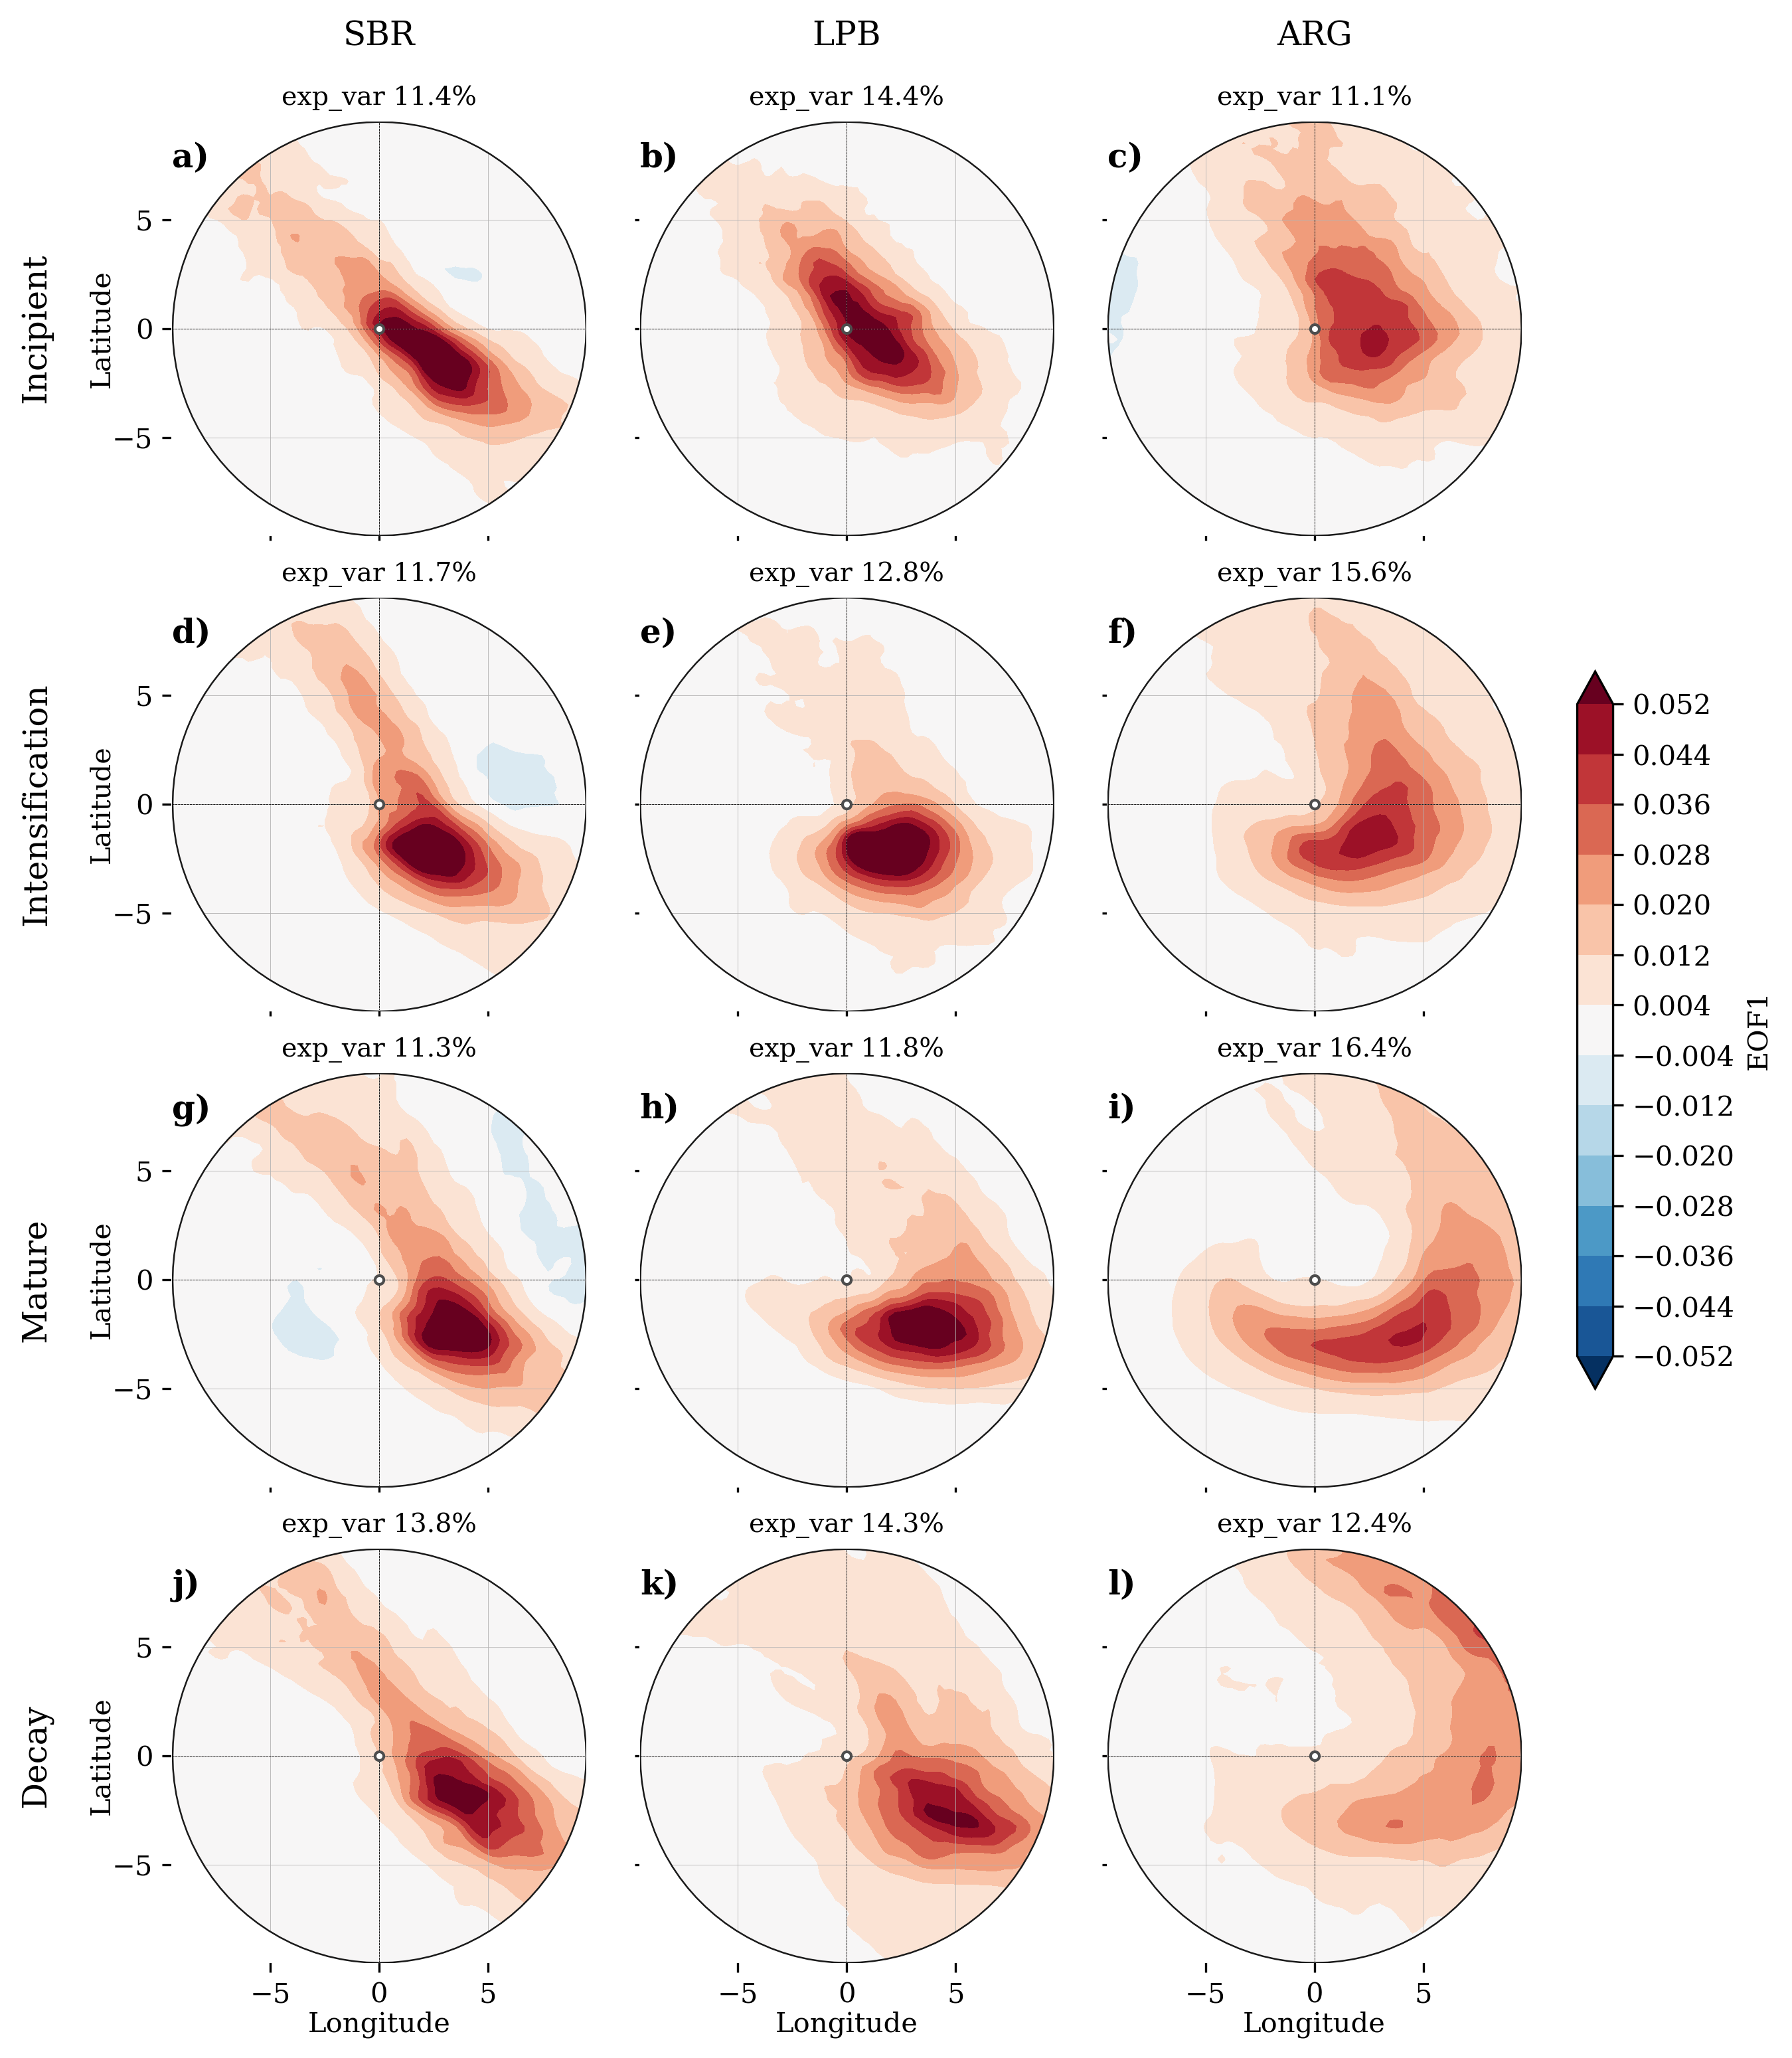
\includegraphics[width=\textwidth]{images/tp/pca1_tp_global_fasesxreg.png}
\caption[EOF1 de precipitação total (População Global)]{Primeiro modo espacial (EOF1) da precipitação total (mm/h) para a População Global de referência. A disposição matricial organiza a evolução por regiões de ciclogênese em colunas (SBR, LPB e ARG) e as fases de desenvolvimento evolutivo em linhas (Incipiente, Intensificação, Maturidade e Decaimento). Sobre cada painel se indica a porcentagem da variância espacial total explicada (\textit{exp\_var}) por essa componente principal. A escala cromática divergente quantifica as anomalias estruturais relativas ao centro do vórtice.}
\label{fig:eof1_tp_global}
\end{figure}

A Figura~\ref{fig:eof1_tp_global} apresenta os padrões espaciais do primeiro modo empírico (EOF1) da precipitação total, com a mesma disposição matricial dos campos PDFe anteriores, um domínio circular centrado no ciclone de 20 graus com contornos que representam anomalias estruturais em relação à média. As porcentagens de variância explicada oscilam entre 11.1\% e 16.4\%, o que indica uma menor dominância do primeiro modo do que no vento a 10~metros.

Em SBR, o EOF1 mantém uma estrutura consistente ao longo do ciclo de vida, com um núcleo positivo máximo ($\sim$0.052) ancorado no quadrante sudeste e uma cauda alongada em direção ao noroeste, formando uma faixa diagonal que atravessa o domínio, a mesma orientação do WCB descrita na Seção~\ref{subsec:kde_tp_global}.

Na fase incipiente (painel a, 11.4\%), o núcleo sudeste coexiste com a cauda noroeste e pequenas zonas negativas ($\sim$$-$0.004 a $-$0.012) no leste. Na intensificação (painel d, 11.7\%), os contornos se tornam mais simétricos e aparece maior área negativa no nordeste, com pequenas zonas negativas fracas. Na maturidade (painel g, 11.3\%), o núcleo positivo se afasta da origem em direção ao sudeste, com valores negativos a oeste e nordeste, também fracos e de pouca extensão. O decaimento (painel j, 13.8\%) mostra aumento de variância e desaparecimento dos valores negativos, resultando em um monopolo positivo puro alongado diagonalmente.

LPB apresenta os padrões mais simétricos e compactos. Na fase incipiente (painel b, 14.4\%), o núcleo positivo máximo ($\sim$0.052) forma uma faixa diagonal noroeste-sudeste, sem valores negativos; sua maior variância nessa fase (14.4\% frente a 11.4\% de SBR e 11.1\% de ARG) indica um modo dominante mais robusto e reprodutível. Na intensificação (painel e, 12.8\%), o núcleo migra para o sudeste com contornos quase perfeitamente simétricos, a simetria mais notável da fase. Na maturidade (painel h, 11.8\%), o núcleo se desloca ligeiramente para leste com contornos alongados. O decaimento (painel k, 14.3\%) mostra aumento de variância, com o núcleo a sudeste e uma cauda positiva em direção ao norte.

ARG exibe o comportamento mais distintivo e assimétrico. Na fase incipiente (painel c, 11.1\%), o núcleo positivo ($\sim$0.052) se localiza no sudeste com elongação ao norte e um dipolo fraco a oeste; sua variância é a mais baixa da figura, refletindo a alta variabilidade não estruturada da região nessa fase, coerente com a estrutura bimodal (núcleo sudeste e foco secundário noroeste) que o PDFe já mostrava para ARG incipiente (Seção~\ref{subsec:kde_tp_global}). A intensificação (painel f, 15.6\%) apresenta o valor mais alto dessa fase na População Global, com o núcleo sudeste mantendo sua posição deslocada e uma cauda norte ausente em SBR e LPB. Diferentemente das regiões oceânicas, em ARG o modo dominante permanece inclinado para o flanco dianteiro mesmo na intensificação. A maturidade (painel i, 16.4\%) alcança o máximo absoluto da figura global, único entre as três regiões, SBR e LPB têm seu pico no decaimento e na fase incipiente, respectivamente, indicando uma organização espacial excepcionalmente reprodutível na Argentina; o núcleo já adota aqui uma forma de arco, que se acentuará no subconjunto p90 (Seção~\ref{subsec:eof1_tp_p90}). O decaimento (painel l, 12.4\%) mostra valores positivos difusos sobre o semicírculo leste sem núcleo definido, contrastando com os padrões mais estruturados de SBR e LPB.

A faixa de anomalias positivas orientada noroeste-sudeste que mostra o EOF1 coincide com a posição dos máximos da PDFe (Seção~\ref{subsec:kde_tp_global}). As anomalias são mais intensas e concentradas em SBR e LPB do que em ARG, o que concorda com a maior intensidade da precipitação nessas regiões (Seção~\ref{sec:pdf_tp}).
Essa baixa variância explicada pelo primeiro modo, consistente com a natureza discontínua da precipitação (Seção~\ref{subsec:var_exp_tp}), constitui a linha de base dispersa que permite dimensionar a transformação estrutural que os eventos p90 experimentam ao se ocluir, quando abandonam esse comportamento transitório para confinar a precipitação em geometrias estruturadas, como se examina a seguir.

\subsection{EOF1 no subconjunto p90}\label{subsec:eof1_tp_p90}

\begin{figure}[htbp]
\centering
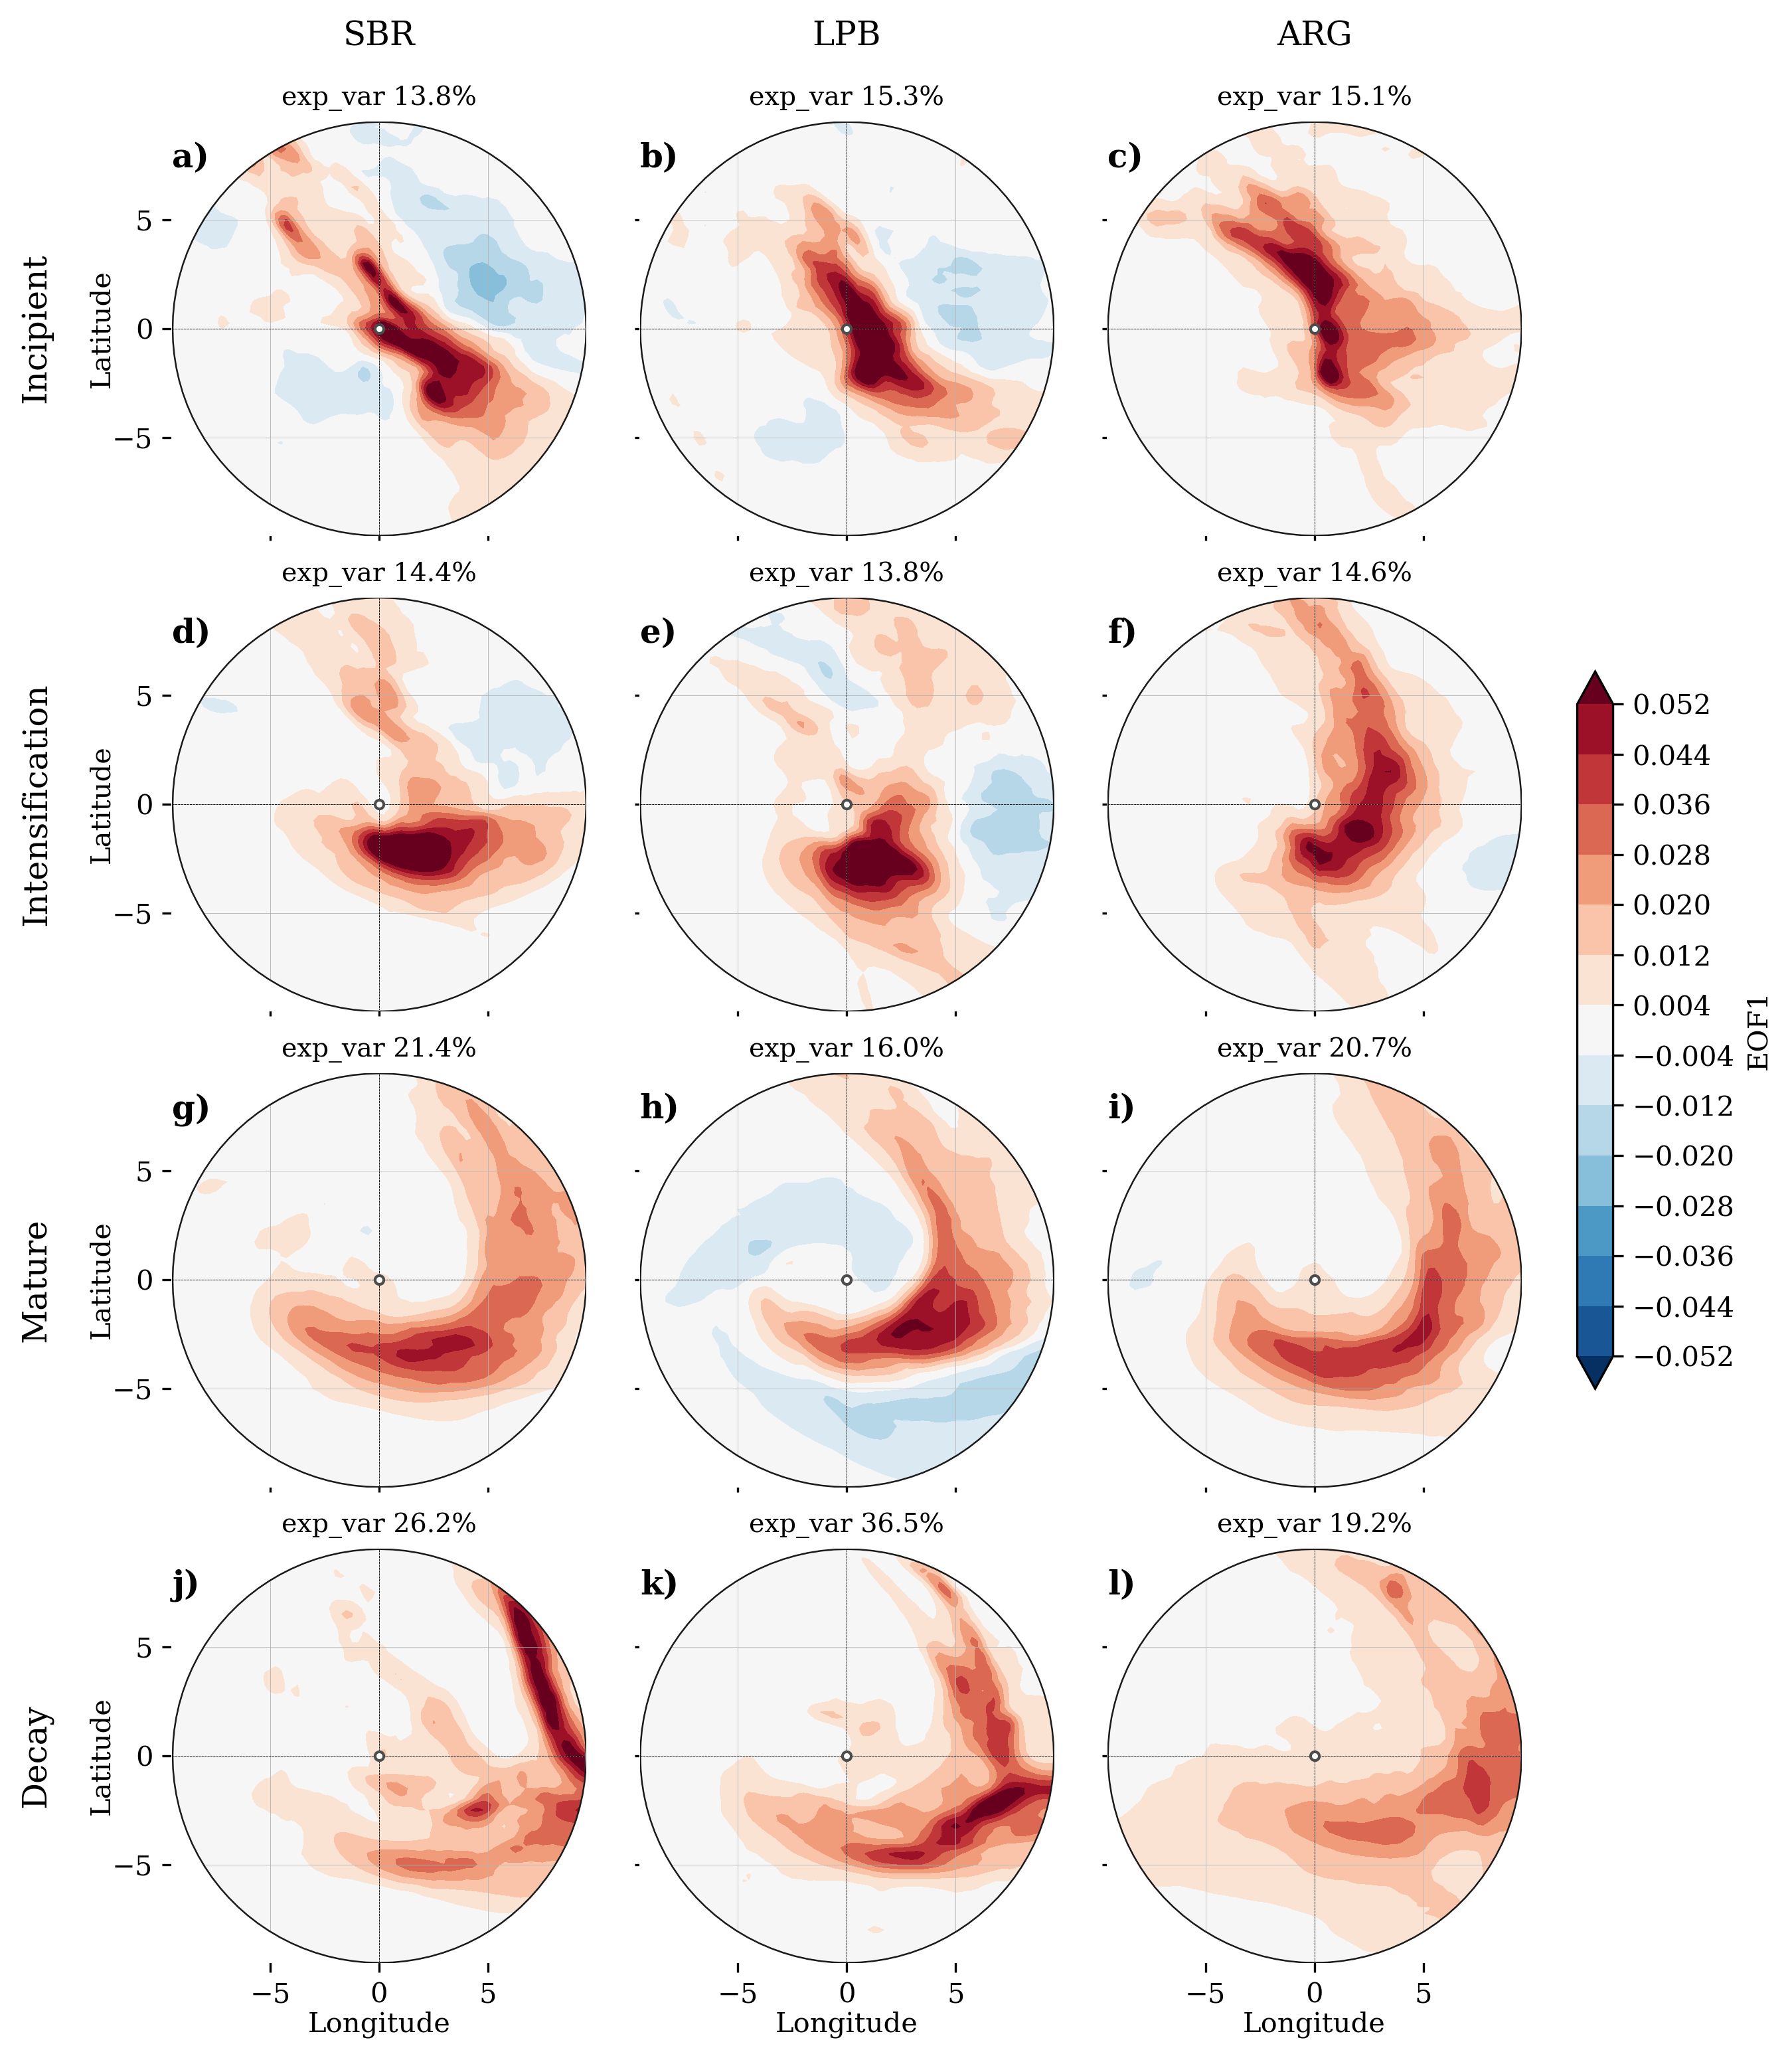
\includegraphics[width=\textwidth]{images/tp/pca1_tp_p90_fasesxreg.png}
\caption[EOF1 de precipitação total (subconjunto p90)]{Primeiro modo espacial (EOF1) da precipitação total (mm/h) para o estrato de ciclones intensos (percentil 90). O formato dos painéis (a--l), a nomenclatura de variância explicada e o domínio espacial mantêm uma correspondência estrita com a Figura~\ref{fig:eof1_tp_global}, permitindo quantificar a profunda transformação estrutural que os sistemas severos experimentam, especialmente durante sua oclusão final.}
\label{fig:eof1_tp_p90}
\end{figure}

A Figura~\ref{fig:eof1_tp_p90} apresenta os padrões espaciais do primeiro modo para o estrato p90, com a mesma disposição matricial da População Global. O contraste com a Figura~\ref{fig:eof1_tp_global} é imediato. A filtragem p90 produz dois efeitos sistemáticos em quase todas as regiões e fases (exceto ARG na intensificação): um incremento generalizado da variância explicada pelo EOF1, mais pronunciado nas fases tardias, e uma transformação morfológica que converte os monopolos e dipolos da população geral em estruturas em arco durante a maturidade e o decaimento.

Durante as fases iniciais, a filtragem p90 refina os padrões do global sem transformá-los radicalmente. Em SBR, a incipiente (painel a, 13.8\%, $+$2.4 pontos) mostra uma faixa diagonal noroeste-sudeste com zonas negativas ($\sim$$-$0.012 a $-$0.028) no nordeste, formando um dipolo mais nítido; a intensificação (painel d, 14.4\%, $+$2.7 pontos) mantém o núcleo próximo à origem, mais compacto, com a zona negativa melhor delimitada. Em LPB, a incipiente (painel b, 15.3\%, $+$0.9 pontos) mantém a faixa diagonal, mais estreita, com zonas negativas semelhantes; a intensificação (painel e, 13.8\%, $+$1.0 pontos) muda de monopolo compacto para dipolo, com o polo positivo ainda a sudeste. Em ARG, a incipiente (painel c, 15.1\%, $+$4.0 pontos) mostra a simplificação mais notável. A faixa diagonal é mais definida do que no global e desaparece o dipolo fraco; a intensificação (painel f, 14.6\%, $-$1.0 pontos) mantém o núcleo sudeste com a cauda norte, com valores negativos mínimos ausentes no global. A intensificação é, em conjunto, a fase mais estável entre global e p90, consistente com a simetria já observada entre ambas as populações no PDFe dessa mesma fase (Seção~\ref{subsec:kde_tp_p90}), o que sugere que os mecanismos de organização durante o desenvolvimento ativo não diferem qualitativamente entre sistemas ordinários e mais intensos.

A maturidade é onde ocorre a transformação morfológica mais drástica. Em SBR (painel g, 21.4\%, $+$10.1 pontos), o padrão do global é substituído por um monopolo positivo em arco do sudoeste até o nordeste, com o quadrante noroeste livre de anomalias positivas, primeira manifestação clara da estrutura em arco como modo dominante. LPB (painel h, 16.0\%, $+$4.2 pontos) forma um arco que envolve o sistema do sudoeste até o nordeste, com zonas negativas ($\sim$$-$0.008 a $-$0.024) no sul e sudeste. ARG (painel i, 20.7\%, $+$4.3 pontos) apresenta um arco semelhante mas de menor extensão e valores negativos mínimos, resultando em um monopolo arqueado sem dipolaridade.

No decaimento, as estruturas se distorcem e se deslocam para o flanco oriental externo. Em SBR (painel j, 26.2\%, $+$12.4 pontos), o núcleo positivo se concentra em uma faixa que margeia o extremo leste do domínio. LPB (painel k, 36.5\%) mostra um arco em forma de "L" invertido do sul até o leste. ARG (painel l, 19.2\%, $+$6.8 pontos) apresenta o padrão mais difuso da linha, semelhante em morfologia ao global, uma desorganização espacial que contrasta com a magnitude, muito mais concentrada. O próprio subconjunto p90 de ARG alcança aqui sua densidade de probabilidade mais alta de toda a Figura~\ref{fig:pdf_tp} (Seção~\ref{sec:pdf_tp}), o que indica que a concentração de magnitude e a organização espacial não são a mesma propriedade.

As estruturas em arco do EOF1 abrangem a zona onde a PDFe localiza os máximos de p90 (Seção~\ref{subsec:kde_tp_p90}), e apareceriam como o padrão dominante de variabilidade espacial se a intrusão seca desloca a umidade do núcleo para a periferia. O EOF1 a quantifica em 21.4\% (SBR) e 20.7\% (ARG) da variância total na maturidade, e 36.5\% (LPB) no decaimento, o que mostra que essa geometria se repete de forma consistente e não se deve a alguns poucos casos isolados.

Ao contrastar com o vento a 10~m, na maturidade os máximos de vento de p90 se concentram no quadrante noroeste, a ${\sim}$2--4° do centro (Seção~\ref{sec:kde_espacial_p90}), enquanto os máximos de precipitação se localizam a leste e sudeste, a ${\sim}$3.5--7° do centro (Seção~\ref{subsec:kde_tp_p90}). Essa separação entre os setores de máximo vento e máxima precipitação é um dos resultados centrais deste capítulo para os ciclones mais intensos.

\subsection{Significância estatística}\label{subsec:significancia_tp}

Para distinguir os sinais físicos das flutuações devidas à amostragem, avalia-se a significância estatística dos padrões espaciais mediante o método Bootstrap-t (Seção~\ref{subsec:bootstrap_significancia}). Como no vento, a análise se concentra na fase de maturidade, que apresenta o maior sinal dinâmico e é a de maior interesse para esta tese. A Figura~\ref{fig:xeof_madurez_global_tp} mostra os três primeiros modos (EOF1--EOF3) e suas componentes principais (PC1--PC3) para a População Global na maturidade, e a Figura~\ref{fig:xeof_madurez_p90_tp} apresenta a análise equivalente para p90. O hachurado indica as áreas significativas a 95\% de confiança.

\begin{figure}[htbp]
\centering
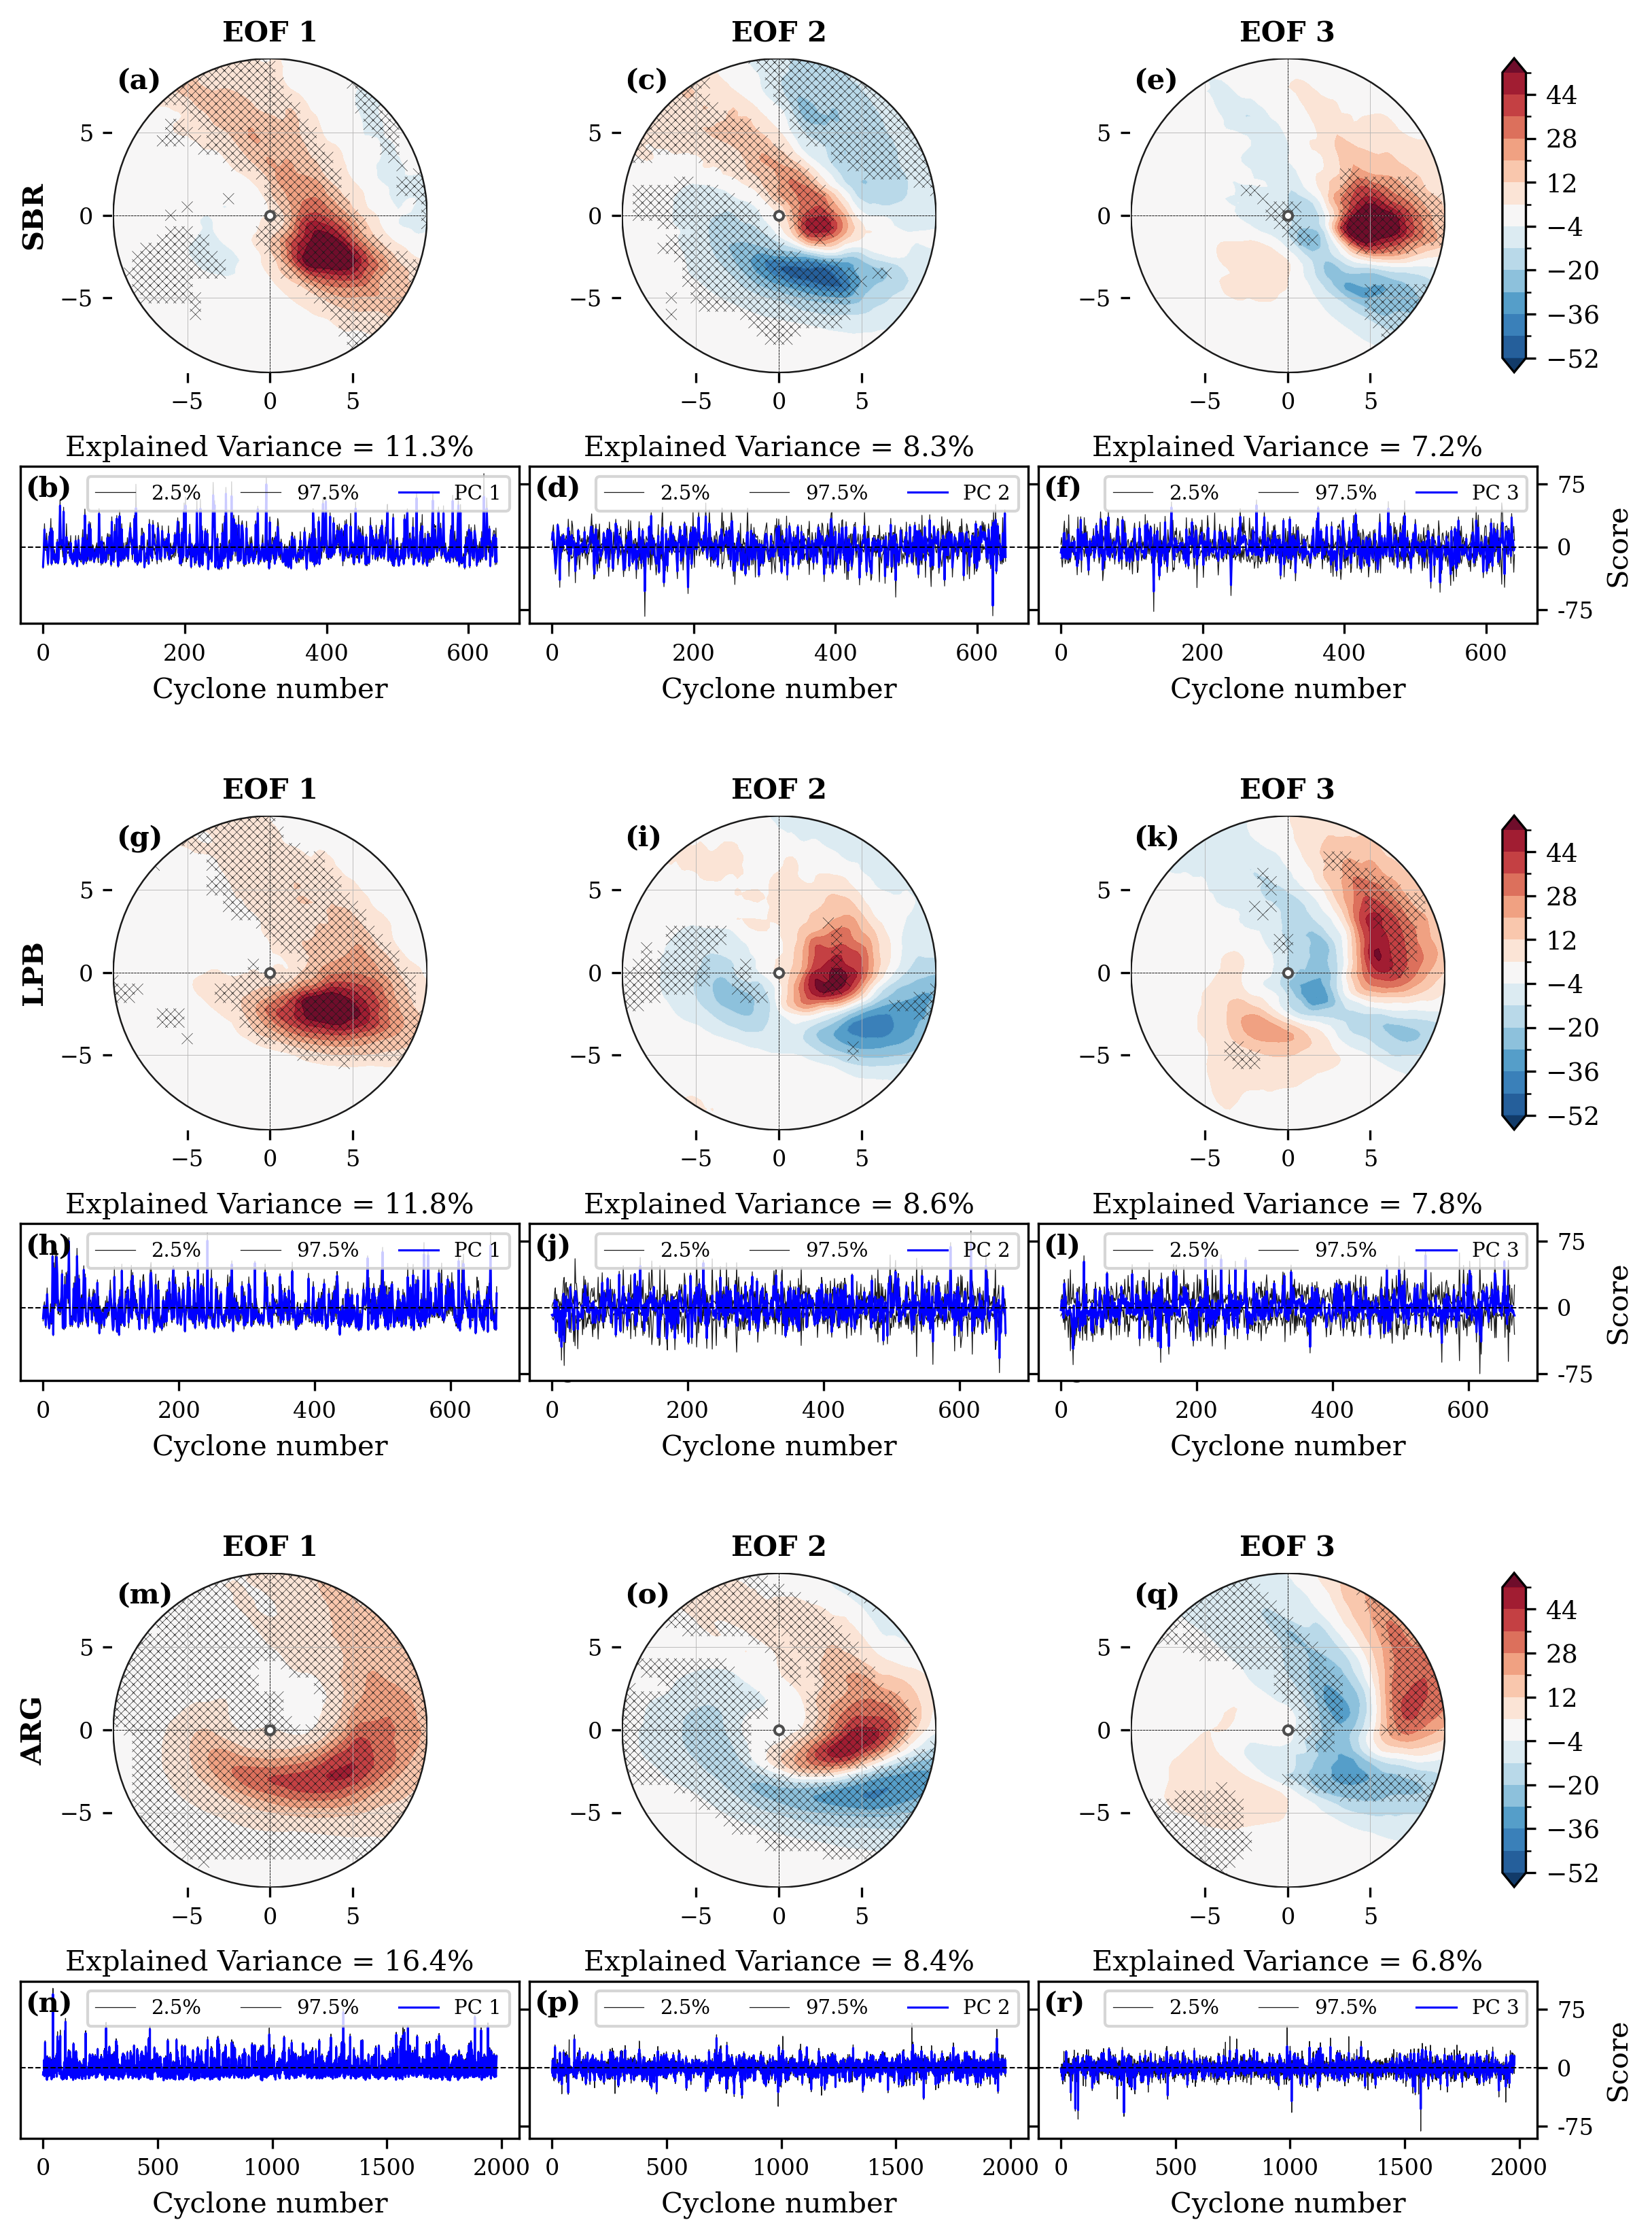
\includegraphics[width=\textwidth]{images/tp/xeof_global_tp_mature.png}
\caption[Significância espacial dos EOFs de precipitação em fase de maturidade (População Global)]{Decomposição EOF da precipitação total para a População Global em fase de maturidade. Painéis (a, g, m): mapas de EOF1 para SBR, LPB e ARG respectivamente; (c, i, o): EOF2; (e, k, q): EOF3. O hachurado indica significância estatística a 95\% (teste Bootstrap-t; Seção~\ref{subsec:bootstrap_significancia}). Painéis (b, h, n): componentes principais PC1; (d, j, p): PC2; (f, l, r): PC3. A linha cinza delimita os percentis 2.5 e 97.5 da distribuição bootstrap.}
\label{fig:xeof_madurez_global_tp}
\end{figure}

\begin{figure}[htbp]
\centering
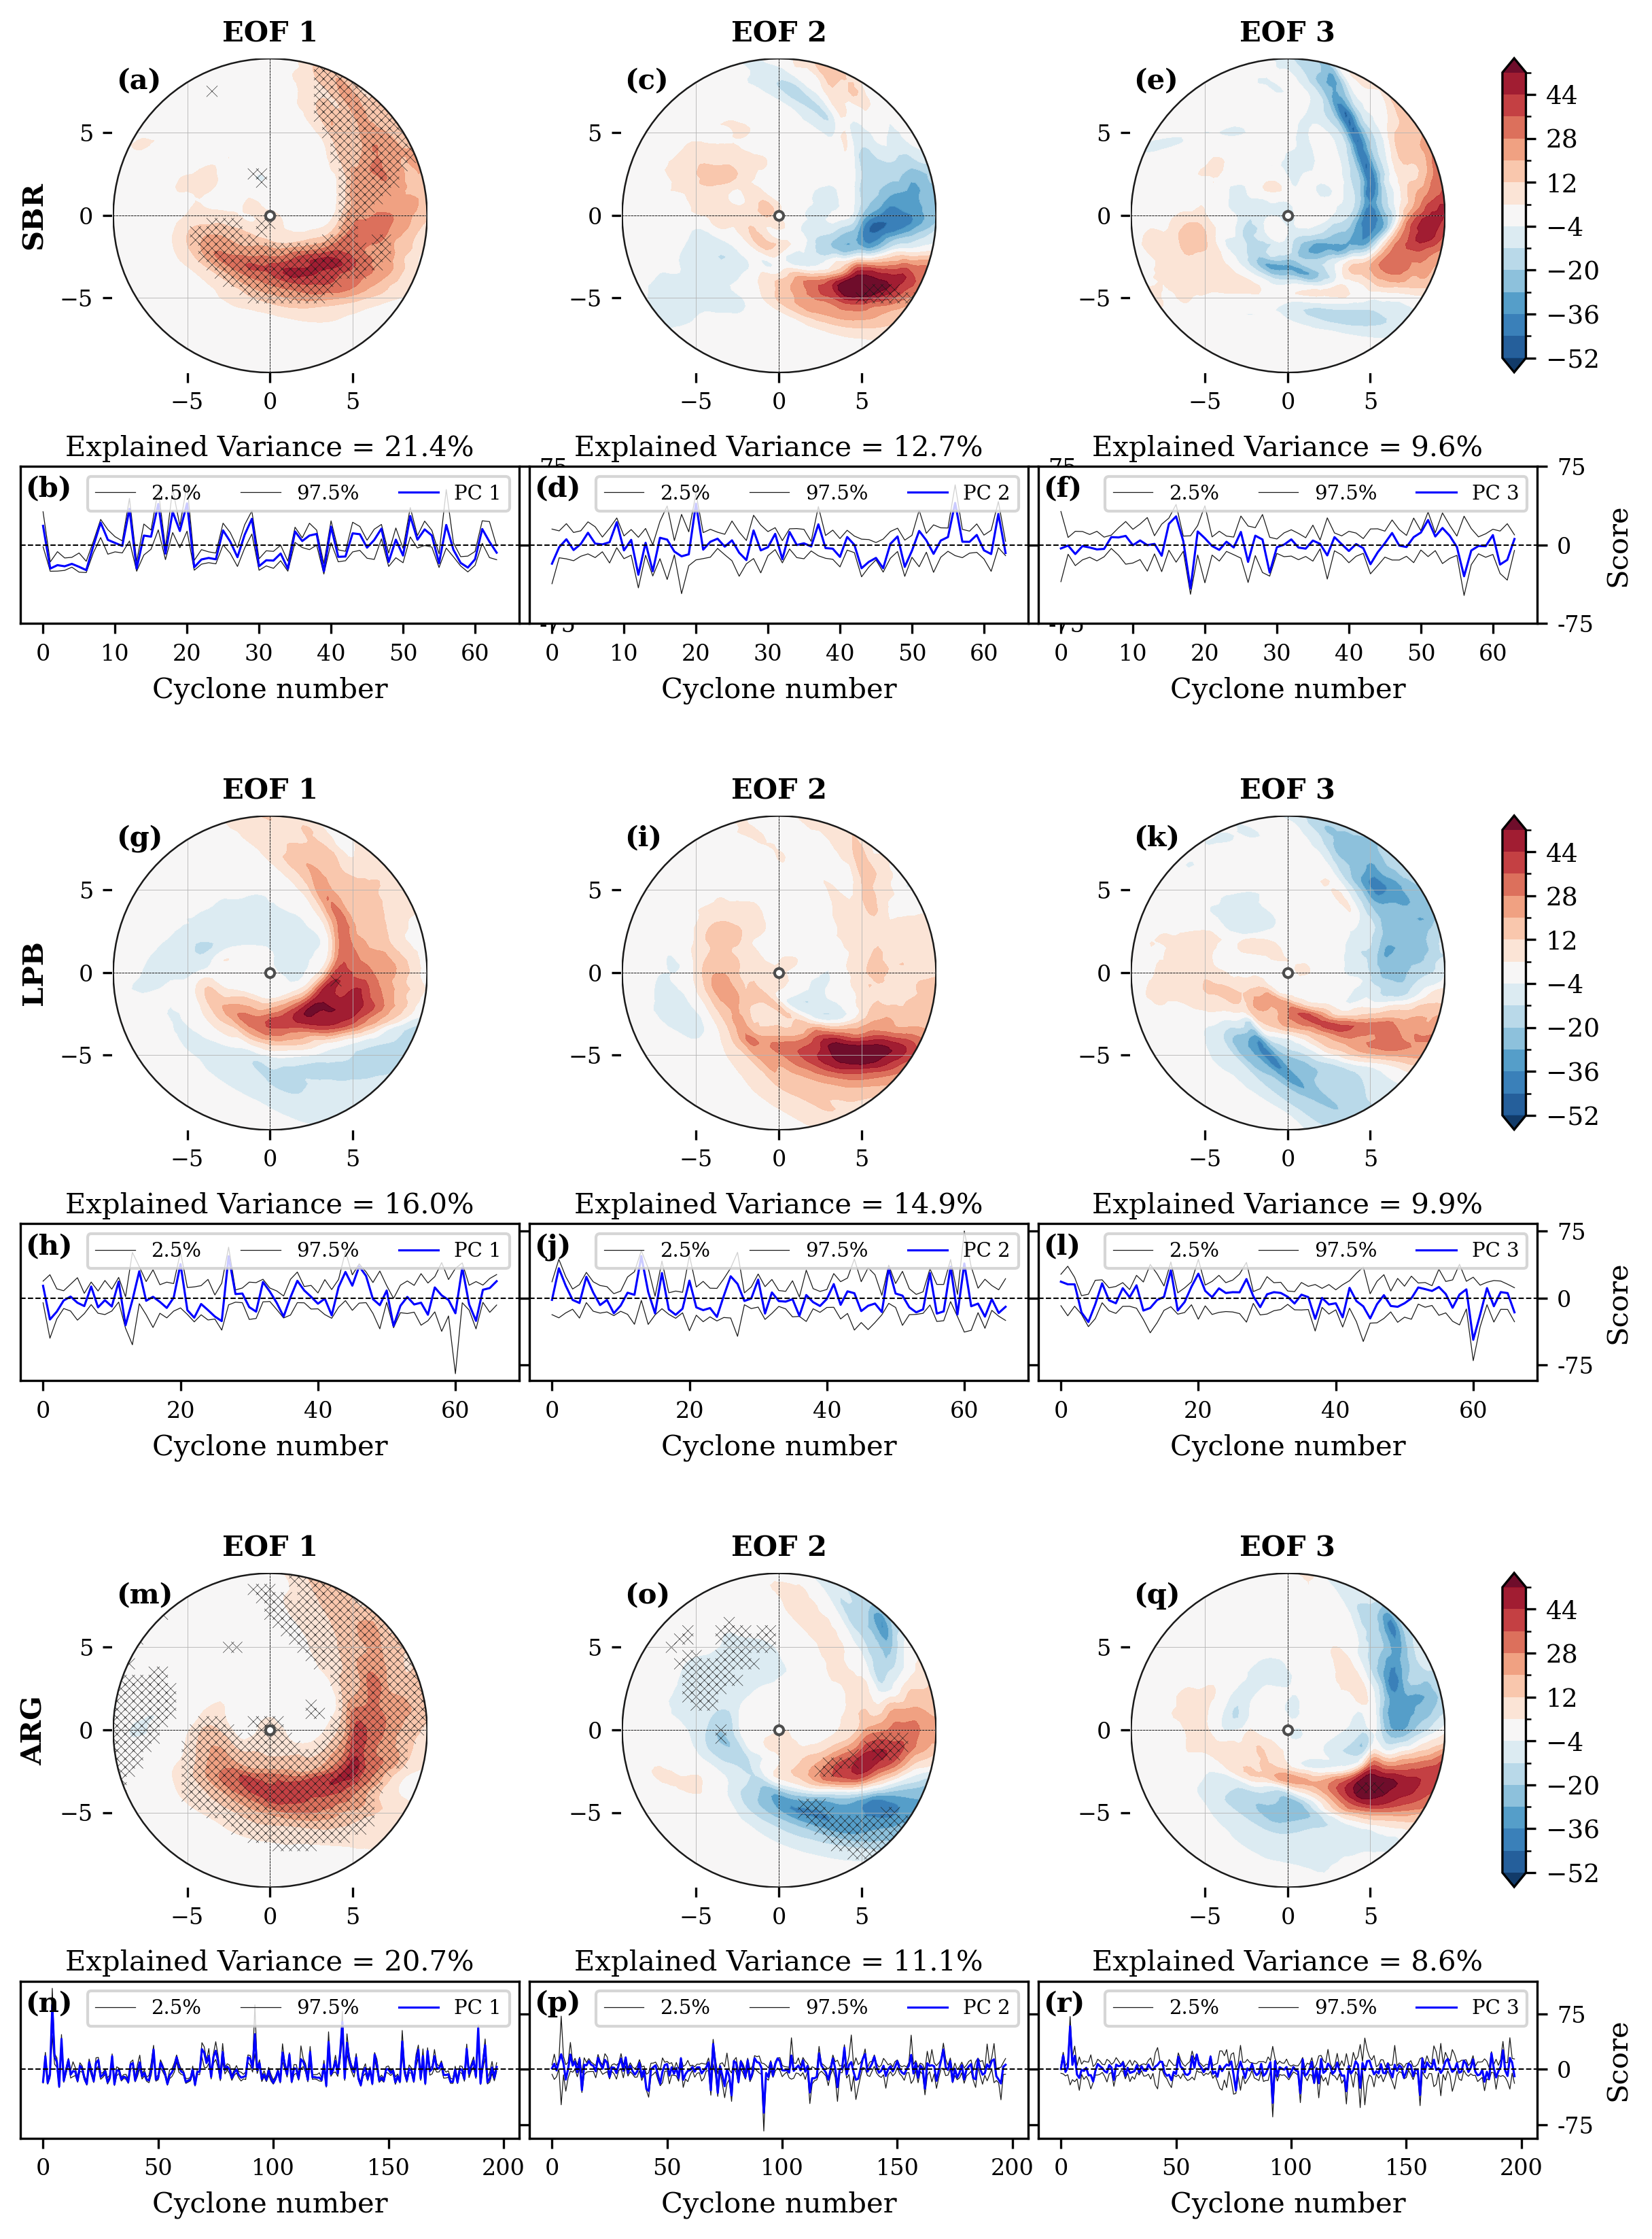
\includegraphics[width=\textwidth]{images/tp/xeof_p90_tp_mature.png}
\caption[Significância espacial dos EOFs de precipitação em fase de maturidade (subconjunto p90)]{Decomposição EOF da precipitação total para o subconjunto extremo (p90) em fase de maturidade. A disposição de painéis é idêntica à Figura~\ref{fig:xeof_madurez_global_tp}.}
\label{fig:xeof_madurez_p90_tp}
\end{figure}

A Figura~\ref{fig:xeof_madurez_global_tp} mostra que, para a População Global na maturidade, as áreas significativas do EOF1 se concentram sobre os valores positivos, sem se estender aos tons próximos de zero. Em SBR, o hachurado segue a faixa diagonal noroeste-sudeste, com alguma significância também no extremo negativo, perto do limite com os tons nulos. Em LPB, o hachurado se restringe à parte mais intensa dessa mesma faixa. Em ARG, o hachurado cobre praticamente todo o domínio, a cobertura mais ampla das três regiões, inclusive sobre tons positivos fracos.
Na Figura~\ref{fig:xeof_madurez_p90_tp}, SBR e ARG mostram um arco de significância denso, que traça a geometria do arco sudoeste-nordeste já identificado no EOF1 (Seção~\ref{subsec:eof1_tp_p90}), consistente com o salto na variância explicada dessa fase. LPB constitui uma excepção notável. Seu salto de variância explicada na maturidade (11.8\% para 16.0\%) é na realidade o mais moderado das três regiões nessa fase, frente aos $+$10.1 pontos de SBR; seu EOF1 carece de área significativa apreciável a 95\%, o que indica que a transformação morfológica em direção à faixa arqueada não é respaldada por um sinal estatisticamente robusto sob o teste Bootstrap-$t$, coerente com a densidade espacial mais baixa que LPB já mostrava no PDFe dessa mesma fase (${\approx}$7--9$\times10^{-4}$, a mais baixa da linha; Seção~\ref{subsec:kde_tp_p90}). As amplitudes de PC2 e PC3 alcançam ou superam em certos casos os limites de confiança bootstrap, o que sugere que mesmo a variabilidade secundária pode ser fisicamente relevante na maturidade dos sistemas mais intensos.

Na Figura~\ref{fig:xeof_madurez_global_tp}, os modos secundários também apresentam áreas significativas, embora de extensão mais limitada do que o EOF1. Em SBR, o EOF2 é significativo tanto em seu polo positivo quanto negativo, com hachurado denso onde o sinal é mais intenso; o EOF3 é significativo principalmente sobre o sinal positivo, com áreas menores perto do centro e no extremo sudeste. Em LPB, o EOF2 apresenta um hachurado mais restrito, limitado aos tons mais intensos do polo positivo e ausente no negativo; o EOF3 tem áreas pequenas que não coincidem com o sinal mais forte. Em ARG, o EOF2 é significativo em ambos os sinais exceto nos valores próximos de zero, e o EOF3 cobre uma área maior do que em LPB, sobre as regiões de sinal mais intenso.

Na Figura~\ref{fig:xeof_madurez_p90_tp}, por sua vez, os modos secundários perdem quase toda sua significância. Em SBR, o EOF2 só conserva uma área pequena perto de seu máximo positivo, e o EOF3 não apresenta áreas significativas. Em LPB, nem o EOF2 nem o EOF3 alcançam significância a 95\%, o que se soma à ausência já apontada em seu EOF1. Em ARG, o EOF2 mostra áreas hachuradas dispersas a noroeste e a sudeste, sem um padrão claro em relação ao sinal, e o EOF3 tampouco é significativo. Esse contraste indica que a filtragem p90, além de concentrar a variância no EOF1 (Seção~\ref{subsec:eof1_tp_p90}), reduz a robustez estatística dos modos secundários, com a possível exceção parcial de ARG.

Essa diferença é coerente com o já apontado para o EOF1 de LPB, cujo salto de variância explicada é o mais moderado das três regiões e cuja densidade espacial no PDFe dessa fase é a mais baixa (Seção~\ref{subsec:kde_tp_p90}), o que sugere um sinal mais fraco e, portanto, mais difícil de distinguir do ruído de amostragem sob o teste Bootstrap-$t$. Em síntese, a estrutura em arco de p90 é respaldada por um sinal estatisticamente robusto em SBR e ARG, mas em LPB continua sendo um padrão morfológico consistente sem confirmação como distinguível do ruído de amostragem.

%%%%%%%%%%%%%%
\section{Componentes principais (PC1--PC3)}\label{sec:dinamica_pc1_tp}

A fragmentação da variância documentada na maturidade e sua transformação em direção à coerência no decaimento têm sua contrapartida temporal no comportamento estatístico das Componentes Principais. Diferentemente do vento, onde as amplitudes de PC2 e PC3 são menores do que as de PC1 na População Global e PC2 se aproxima de PC1 em p90 (Seção~\ref{subsec:res_dinamica_pc1}), na precipitação as amplitudes de PC1, PC2 e PC3 não diferem muito entre si nem entre a População Global e p90. Na precipitação, a correlação entre PC1 e a vorticidade se debilita em magnitude durante a maturidade em LPB, até perder significância; em SBR perde magnitude nessa mesma fase mas se mantém significativa; enquanto em ARG se mantém significativa durante todo o ciclo, com magnitude que se fortalece e depois se debilita ao longo das fases (Seção~\ref{subsec:pc1_global_tp}).

\begin{table}[htbp]
\centering
\caption[Momentos estatísticos e correlação de PC1--PC3 de precipitação - População Global]
{Assimetria ($\gamma_1$) e curtose ($\gamma_2$) da PC1 de precipitação, e correlação de Spearman em valor absoluto ($|r|$) entre PC1, PC2 e PC3 e a vorticidade relativa a 850 hPa associada à fase, para a População Global. Reporta-se o valor absoluto porque o sinal da correlação depende da convenção de sinal arbitrária de cada EOF (Seção~\ref{subsec:analisis_pc}); o relevante é a magnitude da correlação e sua significância. Os valores significativos ($p<0.05$) são mostrados em negrito.}
\label{tab:stat_global_tp}
\begin{tabular*}{\textwidth}{@{\extracolsep{\fill}}llrrrrr}
\hline
\textbf{Região} & \textbf{Fase} & \textbf{Assimetria ($\gamma_1$)} & \textbf{Curtose ($\gamma_2$)} & \textbf{$|$PC1$|$} & \textbf{$|$PC2$|$} & \textbf{$|$PC3$|$} \\
\hline
\textbf{SBR} & Incipiente       & 1.12 & 1.58 & \textbf{0.52} & \textbf{0.16} & \textbf{0.26} \\
             & Intensificação & 0.85 & 0.87 & \textbf{0.52} & \textbf{0.13} & \textbf{0.46} \\
             & Maturidade         & 1.20 & 1.53 & \textbf{0.17} & \textbf{0.65} & 0.04 \\
             & Decaimento     & 1.49 & 2.18 & \textbf{0.19} & \textbf{0.15} & \textbf{0.29} \\
\hline
\textbf{LPB} & Incipiente       & 1.34 & 2.85 & \textbf{0.49} & \textbf{0.10} & 0.07 \\
             & Intensificação & 1.03 & 1.44 & \textbf{0.59} & 0.01 & \textbf{0.33} \\
             & Maturidade         & 1.09 & 1.45 & 0.04 & \textbf{0.61} & \textbf{0.34} \\
             & Decaimento     & 2.06 & 6.02 & 0.07 & \textbf{0.24} & \textbf{0.13} \\
\hline
\textbf{ARG} & Incipiente       & 2.55 & 9.30 & \textbf{0.51} & \textbf{0.18} & 0.04 \\
             & Intensificação & 1.52 & 4.06 & \textbf{0.66} & \textbf{0.26} & \textbf{0.22} \\
             & Maturidade         & 1.74 & 5.40 & \textbf{0.53} & \textbf{0.43} & 0.04 \\
             & Decaimento     & 2.50 & 9.59 & \textbf{0.25} & 0.00 & \textbf{0.13} \\
\hline
\end{tabular*}
\end{table}


\subsection{Relação com a intensidade na População Global}\label{subsec:pc1_global_tp}

A Tabela~\ref{tab:stat_global_tp} documenta a assimetria e a curtose da PC1, e a correlação de Spearman em valor absoluto entre PC1, PC2 e PC3 e a vorticidade relativa a 850~hPa associada à fase, para a População Global, desagregadas por região e fase.

A análise dos momentos estatísticos revela uma característica distintiva, a presença persistente de caudas pesadas (leptocurtose positiva) ao longo de todo o ciclo de vida. Diferentemente do vento, onde a curtose evoluía para valores próximos de zero ou negativos na maturidade, aqui se observam valores de $\gamma_2$ positivos nas três regiões: SBR oscila entre $+0.87$ (intensificação) e $+2.18$ (decaimento); LPB exibe curtose pronunciada na incipiência ($+2.85$) e no decaimento ($+6.02$); ARG apresenta os valores mais extremos, superiores a $+9$ tanto na incipiência quanto no decaimento. O sesgo positivo persistente ($\gamma_1 > +0.8$ em todos os casos) reflete a presença de eventos com anomalias pluviométricas intensas em relação ao padrão médio.

O exame das correlações entre PC1 e vorticidade revela uma evolução distinta por região durante a maturidade. Em SBR, a correlação moderada das fases iniciais ($|r|\approx0.52$) perde magnitude até a maturidade ($|r|=0.17$) e o decaimento ($|r|=0.19$), embora se mantenha significativa em ambas as fases. Em LPB, as correlações significativas durante o desenvolvimento ($|r|=0.49$ na incipiência, $0.59$ na intensificação) colapsam para valores não significativos na maturidade ($|r|=0.04$, $p=0.26$) e no decaimento ($|r|=0.07$, $p=0.07$). ARG mantém correlações significativas durante todo o ciclo, com um fortalecimento inicial até a intensificação ($|r|=0.66$) e um debilitamento posterior até o decaimento ($|r|=0.25$).

Esse comportamento reflete processos físicos diferenciados. Em SBR, a correlação perde magnitude até a maturidade e o decaimento, embora se mantenha significativa; em LPB, as correlações significativas do desenvolvimento colapsam para valores não significativos na maturidade e no decaimento. Em ARG, a correlação se mantém significativa durante todo o ciclo (Seção~\ref{subsec:pc1_global_tp}), o que é consistente com o fato de seu EOF1 ser, na População Global, o modo mais dominante e reprodutível das três regiões, com o máximo absoluto de variância explicada de toda a figura na maturidade (16.4\%, Seção~\ref{subsec:eof1_tp_global}). Em SBR e LPB, por sua vez, o EOF1 explica uma fração menor da variância justamente nessa fase (11.3\% e 11.8\%, respectivamente, Seção~\ref{subsec:var_exp_tp}), o que poderia tornar sua correlação com a vorticidade mais frágil.

O debilitamento de PC1 na maturidade não implica que a vorticidade deixe de organizar o campo de precipitação, em SBR e LPB o sinal de maior magnitude se desloca para PC2. Em SBR, PC2 alcança $|r|=0.65$ na maturidade, uma magnitude maior do que a do próprio PC1 nessa mesma fase ($|r|=0.17$); em LPB ocorre algo equivalente, PC2 chega a $|r|=0.61$ na maturidade, justamente quando PC1 perde significância ($|r|=0.04$). Esse revezamento entre modos sugere que, ao se ocluir o sistema e suprimir-se a convecção do núcleo, a parte da estrutura pluviométrica que continua escalando com a intensidade deixa de ser a dominante (EOF1) e passa a ser uma estrutura secundária (EOF2), sem que a correlação entre precipitação e vorticidade desapareça por completo.

\begin{table}[htbp]
\centering
\caption[Momentos estatísticos e correlação de PC1--PC3 de precipitação - Subconjunto p90]
{Assimetria ($\gamma_1$) e curtose ($\gamma_2$) da PC1 de precipitação, e correlação de Spearman em valor absoluto ($|r|$) entre PC1, PC2 e PC3 e a vorticidade relativa a 850 hPa associada à fase, para o subconjunto extremo (p90). Reporta-se o valor absoluto porque o sinal da correlação depende da convenção de sinal arbitrária de cada EOF (Seção~\ref{subsec:analisis_pc}); o relevante é a magnitude da correlação e sua significância. Os valores significativos ($p<0.05$) são mostrados em negrito.}
\label{tab:stat_p90_tp}
\begin{tabular*}{\textwidth}{@{\extracolsep{\fill}}llrrrrr}
\hline
\textbf{Região} & \textbf{Fase} & \textbf{Assimetria ($\gamma_1$)} & \textbf{Curtose ($\gamma_2$)} & \textbf{$|$PC1$|$} & \textbf{$|$PC2$|$} & \textbf{$|$PC3$|$} \\
\hline
\textbf{SBR} & Incipiente       & 1.57 & 3.48  & \textbf{0.36} & \textbf{0.53} & 0.22 \\
             & Intensificação & 1.20 & 1.67  & \textbf{0.48} & \textbf{0.43} & 0.24 \\
             & Maturidade         & 0.41 & -0.67 & 0.17 & 0.22 & 0.11 \\
             & Decaimento     & 4.02 & 19.77 & \textbf{0.34} & 0.17 & 0.18 \\
\hline
\textbf{LPB} & Incipiente       & 1.90 & 4.52  & \textbf{0.49} & \textbf{0.31} & 0.22 \\
             & Intensificação & 0.60 & -0.38 & \textbf{0.43} & 0.01 & \textbf{0.26} \\
             & Maturidade         & 0.56 & 0.16  & 0.03 & 0.18 & 0.02 \\
             & Decaimento     & 4.34 & 23.18 & \textbf{0.50} & 0.09 & 0.03 \\
\hline
\textbf{ARG} & Incipiente       & 4.43 & 30.88 & \textbf{0.44} & \textbf{0.29} & \textbf{0.23} \\
             & Intensificação & 1.87 & 5.15  & \textbf{0.37} & \textbf{0.21} & \textbf{0.28} \\
             & Maturidade         & 1.66 & 4.53  & \textbf{0.24} & 0.03 & 0.14 \\
             & Decaimento     & 1.96 & 3.37  & \textbf{0.39} & \textbf{0.32} & 0.10 \\
\hline
\end{tabular*}
\end{table}


\subsection{Relação com a intensidade no subconjunto p90}\label{subsec:pc1_p90_tp}

A Tabela~\ref{tab:stat_p90_tp} expõe os parâmetros estatísticos e as correlações (PC1--PC3, em valor absoluto) para o subconjunto extremo. Diferentemente da leptocurtose persistente da População Global, aqui se documenta uma evolução não monotônica em direção a valores extremos no decaimento, junto com um colapso da correlação de PC1 em SBR e LPB durante a maturidade.

Em SBR observa-se leptocurtose alta nas fases iniciais ($\gamma_2 = +3.48$ na incipiência, $+1.67$ na intensificação), seguida de uma curtose próxima de zero na maturidade ($\gamma_2 = -0.67$, sem caudas pronunciadas) e muito alta no decaimento ($\gamma_2 = +19.77$, $\gamma_1 = +4.02$). LPB reproduz esse padrão com valores ainda mais extremos: curtose de $+4.52$ na incipiência, próxima de zero na maturidade ($\gamma_2 = +0.16$) e superior a $+23$ no decaimento. ARG apresenta a curtose mais elevada do conjunto na incipiência ($\gamma_2 = +30.88$), com valores positivos durante todo o ciclo, embora decrescentes após essa fase ($+5.15$ na intensificação, $+4.53$ na maturidade, $+3.37$ no decaimento). Em ARG, essa curtose tão alta na fase incipiente é consistente com a maior heterogeneidade estrutural que caracteriza essa fase (Seção~\ref{subsec:tb_fases}), acentuada por um mecanismo de gênese a sotavento dos Andes (Seção~\ref{subsec:tb_arg}), mais variável do que o forçamento termodinâmico oceânico que organiza a gênese em SBR e LPB. A maioria dos sistemas incipientes de ARG projeta-se fracamente sobre o EOF1, enquanto alguns poucos casos, com amplitudes muito mais altas e alinhados com a geometria do modo dominante, geram a cauda pesada que eleva a curtose observada. Essa leitura é coerente com o apontado na Seção~\ref{subsec:eof1_tp_p90}, onde o EOF1 de ARG na fase incipiente de p90 apresenta o maior salto de variância explicada entre as três regiões nessa fase ($+$4.0 pontos) e perde o dipolo fraco presente na População Global, o que indica que a filtragem p90 retém principalmente os casos melhor alinhados com o modo dominante.

As correlações de PC1 com a vorticidade colapsam durante a maturidade em SBR ($|r|=0.17$, não significativo) e LPB ($|r|=0.03$, $p = 0.80$), recuperando-se no decaimento ($|r|=0.34$ e $0.50$ respectivamente), enquanto ARG mantém valores significativos ainda que atenuados ($|r|=0.24$ na maturidade).

Esse colapso é consistente com a defasagem de fases já documentada (Seção~\ref{sec:pdf_tp}). Em p90, o máximo de precipitação tende a ocorrer antes do máximo de intensidade dinâmica, e quando o vórtice alcança sua vorticidade extrema na maturidade, o núcleo poderia já ter secado pela chegada de ar subsidente, como se propôs nessa mesma seção, de modo que a vorticidade extrema já não coincidiria temporalmente com uma fase ativa de geração de precipitação.

Os modos secundários em p90 não reproduzem o padrão de revezamento observado na População Global. PC2 é significativo principalmente nas fases iniciais (incipiente e intensificação) nas três regiões, com magnitudes de $|r|$ entre $0.32$ e $0.53$, mas não recupera especificamente o sinal que PC1 perde na maturidade. Isso sugere que, nos sistemas mais intensos, o debilitamento do vínculo entre precipitação e vorticidade durante a maturidade é mais generalizado do que na População Global, sem que um único modo secundário assuma o papel que PC1 deixou.

Em SBR e LPB, a perda de correlação durante a maturidade ocorre ao mesmo tempo que a separação espacial documentada nas seções anteriores. Uma vez que a estrutura em arco domina o campo, a amplitude da PC1 já não depende da profundidade do vórtice, mas de quanto dessa faixa permanece dentro do domínio centrado no sistema à medida que o ciclone se dissipa, o que poderia explicar a evolução para a normalidade estatística na maturidade seguida da curtose muito alta no decaimento. Essa hipótese é coerente com a localização dos núcleos de p90 nessas fases (Seção~\ref{subsec:kde_tp_p90}), que na maturidade se situam perto da borda do domínio em SBR (${\sim}$6--7° a leste) e no decaimento se afastam ainda mais, com os contornos de LPB alcançando $+$9° de longitude, praticamente o limite do domínio de 20°×20°. Em LPB essa leitura deve ser tomada com cautela, pois, diferentemente de SBR, sua estrutura em arco em p90-maturidade é morfologicamente clara mas não alcança significância estatística a 95\% (Seção~\ref{subsec:significancia_tp}), de modo que o mecanismo proposto descreve um padrão consistente antes do que uma estrutura já confirmada como robusta frente à amostragem.

A persistência de correlações significativas em ARG durante toda a evolução é consistente com a maior dominância e reprodutibilidade de seu EOF1 já apontadas (Seção~\ref{subsec:pc1_global_tp}), e com a menor magnitude de precipitação de ARG em relação a SBR e LPB já documentada no PDF (Seção~\ref{sec:pdf_tp}).
Esses resultados mostram que o campo de precipitação é estruturalmente mais complexo do que o cinemático. A combinação de distribuições variáveis, correlações que colapsam e se recuperam, e diferenças regionais notáveis indica que a vorticidade não é suficiente para descrever a precipitação durante a fase crítica de maturidade nas regiões oceânicas, onde a separação espacial é mais pronunciada. Isso é coerente com o que \citet{corner2025classification} encontram em escala mais amplia, uma correlação apenas moderada ($r = 0.47$) entre precipitação e vorticidade relativa, que atribuem ao aquecimento diabático e seu efeito sobre a anomalia de vorticidade potencial em níveis baixos.

\section{Síntese}\label{sec:sintesis_tp}

A análise do campo de precipitação total mostra que a arquitetura pluviométrica evolui de um regime de dispersão frontal para um de concentração ocluída, segundo a intensidade dinâmica do sistema.

\paragraph{Magnitude.}
Na População Global, SBR e LPB mostram perfis largos e planos com pico modal próximo de 20~mm/h; ARG concentra seu pico em valores baixos (${\sim}$5--6~mm/h). No subconjunto p90, o pico se desloca para valores um pouco maiores durante as fases iniciais (${\sim}$25~mm/h em SBR incipiente, ${\sim}$30~mm/h em LPB intensificação), embora as taxas superiores a 60~mm/h não sejam exclusivas de p90. Essa relação se inverte na maturidade e no decaimento, a População Global de SBR e LPB se desloca para valores baixos (${\sim}$17 e ${\sim}$10~mm/h na maturidade, ${\sim}$5~mm/h no decaimento), e p90 se concentra em magnitudes ainda menores (1--4~mm/h, densidade ${\sim}$0.18 em SBR). Esse padrão mostra que, a partir da maturidade, pertencer ao subconjunto mais intenso dinamicamente (p90) deixa de implicar maior magnitude de precipitação, e inclusive ocorre o contrário.

\paragraph{Localização.}
Na População Global, os máximos se organizam com assimetria persistente em direção ao setor oriental e sudeste, em uma posição coincidente com a que a literatura atribui à precipitação do WCB (Seção~\ref{subsec:kde_tp_global}), com densidades máximas de ${\sim}$23--25$\times10^{-4}$ em SBR durante a intensificação. No subconjunto p90, essa organização muda ao alcançar a maturidade. Os máximos se afastam do centro e se confinam em faixas alongadas em direção ao leste e sudeste, cuja posição coincide mais com a precipitação associada ao WCB do que com o quadrante ocluso do modelo de Shapiro-Keyser (Seção~\ref{subsec:kde_tp_p90}). No decaimento, essa faixa persiste ancorada ao flanco sudeste e oriental (SBR: ${\sim}$5--7$\times10^{-4}$; LPB: contornos que alcançam $+$9° de longitude), enquanto na População Global o sinal se dissipa. Nos ciclones mais intensos, os máximos de vento se concentram no quadrante noroeste (Capítulo~\ref{cap:resultados_wind10}), enquanto os máximos de precipitação se organizam a leste e sudeste, configurando uma separação espacial entre os forçantes cinemático e hidrológico do sistema.

\paragraph{Padrões de variabilidade.}
Na População Global, a variância espacial se distribui entre múltiplos modos, com o EOF1 explicando apenas entre 11.1\% e 16.4\% da variância total, consistente com a natureza discontínua da precipitação. No subconjunto p90, o EOF1 se concentra abruptamente durante a maturidade e o decaimento, alcançando seu máximo em LPB (36.5\% no decaimento, $+$22.2 pontos em relação ao global) e valores comparáveis em SBR (26.2\% no decaimento), um salto sem equivalente no campo de vento. Esse salto poderia refletir que uma mesma estrutura espacial, o arco, se repete em muitos dos casos mais intensos, possivelmente porque a intrusão seca desloca a atividade pluviométrica para a periferia.

\paragraph{Relação com a intensidade.}
Na População Global, a correlação entre PC1 e a vorticidade associada à fase é moderada nas fases iniciais nas três regiões ($|r|\approx0.5$), o que indica um vínculo real entre o padrão dominante e a intensidade do ciclone. Até a maturidade, esse vínculo evolui de forma distinta em cada região. Em LPB, $|r|$ se aproxima de zero e deixa de ser significativo, o padrão deixa de estar associado à vorticidade. Em ARG, $|r|$ se mantém distante de zero e significativo durante todo o ciclo, embora se debilite até o decaimento, consistente com a maior dominância de seu EOF1 na População Global (Seção~\ref{subsec:pc1_global_tp}). Em SBR, a correlação perde magnitude até a maturidade, embora se mantenha significativa ($|r|=0.17$). Em SBR e LPB, essa perda de sinal em PC1 é compensada parcialmente por PC2, que alcança $|r|=0.65$ e $|r|=0.61$ respectivamente na maturidade, uma magnitude maior do que a do próprio PC1 nessa fase. No subconjunto p90, a correlação de PC1 com a vorticidade colapsa durante a maturidade em SBR ($|r|=0.17$, não significativo) e LPB ($|r|=0.03$, $p = 0.80$), recuperando-se parcialmente no decaimento ($|r|=0.34$ e $0.50$, respectivamente); ARG mantém correlações significativas ainda que atenuadas durante todo o ciclo ($|r|=0.24$ na maturidade), e a perda de correlação entre vorticidade e precipitação em SBR e LPB é mais pronunciada durante a maturidade do que em ARG. Diferentemente da População Global, em p90 os modos secundários não recuperam especificamente o sinal perdido na maturidade, embora sejam significativos nas fases iniciais. Em SBR e LPB, isso mostra que, nos ciclones mais intensos, a vorticidade do centro deixa de prever como se organiza a precipitação. É coerente com o que documenta \citet{shapiro1999bridge} durante a oclusão, ar seco a oeste do centro e precipitação deslocada para leste (Seção~\ref{sec:pdf_tp}).

\paragraph{Alcance.}
Esses resultados dependem da vorticidade de cada fase como medida pontual de intensidade e poderiam diferir com uma medida integrada de circulação \citep{sinclair1997objective}. Além disso, o ERA5 tende a subestimar a precipitação dos ciclones mais intensos em torno de 23\% \citep{chen2024evaluation} (Seção~\ref{sec:datos_era5}), e a distinção entre a faixa leste-sudeste observada em p90 e o quadrante ocluso do modelo de Shapiro-Keyser se apoia em estudos de ciclones do Hemisfério Norte \citep{martin1999forcing, sawada2021heavy} e na simetria entre hemisférios, sem um estudo equivalente para o Atlântico Sul. A intrusão seca proposta como mecanismo de reorganização tampouco é medida diretamente, e é uma das explicações que o Capítulo~\ref{cap:resultados_wind10} (Seção~\ref{subsec:eof1_wind10_p90}) tampouco consegue distinguir do CCB e do \textit{sting jet} para o núcleo de vento do quadrante noroeste.

Essa base empírica sobre a precipitação, em particular a descrição por fases da separação espacial entre vento e chuva, fornece o alicerce para a análise combinada mediante EOF multivariado (MEOF; Seção~\ref{subsec:eof_multivariado}) no capítulo seguinte, onde a covariância conjunta de ambos os campos é sintetizada nos protótipos estruturais descritos na Seção~\ref{subsec:prototipos}.
